\input{preamble.tex}
\addbibresource{biblio.bib}

\newacronym{bcis}{BCIs}{Interfaces Cerebro-Computador}
\newacronym{bci}{BCI}{Interfaz Cerebro-Computador}
\newacronym{cnn}{CNN}{Red Neuronal Convolucional}
\newacronym{cns}{CNS}{Sistema Nervioso Central}
\newacronym{eeg}{EEG}{Electroencephalography}
\newacronym{erp}{ERP}{Event-Related Potentials}
\newacronym{mi}{MI}{Motion Imagery}
\newacronym{mrcp}{MRCP}{Movement-Related Cortical Potential}
\newacronym{oms}{OMS}{Organización Mundial de la Salud}
\newacronym{sci}{SCI}{Lesion de la médula Espinal}
% ---------------------------------------------- % 


%%%%%%%%%%%% - INICIO DEL DOCUMENTO - %%%%%%%%%%%%

\begin{document} 


% %%%%%%%%%%%% -  PORTADA %%%%%%%%%%%%
%%%%%%%%%%%% -  INICIO PORTADA %%%%%%%%%%%%
% cover page

\definecolor{BLACK}{rgb}{0,0,0} 
\definecolor{MUII}{rgb}{0,0,0.5}
\definecolor{MUIT}{rgb}{0.6,0.2,0.0}
\definecolor{GIM}{rgb}{0.4,0.0,0.2}
\definecolor{GIE}{rgb}{0.01,0.4,0.01}
\definecolor{GIEAI}{rgb}{0.25,0.25,0.25}
\definecolor{GITT}{rgb}{0.0,0.0,0.0}
\definecolor{GIITI}{rgb}{0.2,0.4,1}
\definecolor{WHITE}{rgb}{1,1,1}

\thispagestyle{empty}
%INDICAR EL COLOR CORRESPONDIENTE A LA TITULACIÓN
\pagecolor{WHITE}\afterpage{\nopagecolor}
{\Large
\begingroup
    \begin{center}
        \textcolor{BLACK}{UNIVERSIDAD MIGUEL HERNÁNDEZ DE ELCHE}
         \textcolor{BLACK}{MÁSTER UNIVERSITARIO EN ROBÓTICA} \\
    \end{center}
\endgroup
}

\vspace{50pt}

\begin{center}
    
\includegraphics[width=0.25\columnwidth]{img/logo_umh_round_bw.png}
\end{center}

\vspace{30pt}
{\large
\begingroup
    \begin{center}
        \textcolor{BLACK}{REDES NEURONALES CONVOLUCIONALES PARA EL ANÁLISIS DE SEÑALES EEG DURANTE LA MARCHA CON UN EXOESQUELETO}
    \end{center}
\endgroup
}
\vspace{40pt}

{\large
\begingroup
     \begin{center}
        \textcolor{BLACK}{TRABAJO FIN DE MÁSTER} \\
        \textcolor{BLACK}{Mayo - 2026} \\
    \end{center}
\endgroup
}
\vspace*{\fill}


{\large
\begingroup
    \begin{flushright}

        \begin{tabular}{rl}
        \textcolor{BLACK}{AUTOR:} & \textcolor{BLACK}{Daniel Rosique Egea} \\
        \textcolor{BLACK}{DIRECTOR:} & \textcolor{BLACK}{Eduardo Iañez Martinez}
        \end{tabular}

    \end{flushright}
\endgroup}

%%%%%%%%%%%% -  FINAL PORTADA %%%%%%%%%%%%
% %%%%%%%%%%%% -  FINAL PORTADA %%%%%%%%%%%%
\afterpage{\blankpage} % Se añade una página en blanco después de la cita.
\newpage
\thispagestyle{plain}

%%%%%%%%%%%%%%%%%%%%%%%%%%%%%%%%%%%%%%%%%%%%%%%%%%

% Las páginas anteriores al contenido del TFG/TFM (previas a la introducción) suelen numerarse de forma distinta a las del cuerpo del informe, en este caso en números romanos:
\pagenumbering{roman}

%%%%%%%%%%%%%%%%%%%%%%%%%%%%%%%%%%%%%%%%%%%%%%%%%%


%%%%%%%%%%%%%$%%%%% - CITA - %%%%%%%%%%%%%%%%%%%%%
 
% Se comienza una página nueva sin formato (sin número de página y sin encabezado/pie de página), ya que sólo incorpora la cita:
\newpage
\thispagestyle{empty}

\begin{flushright} % Se alinea el texto en el lado derecho de la página.
\vspace*{5cm} % Se añade un espacio vertical de 5cm para situar la cita en ~1/3 de la página.

\textit{“The human brain, sculpted by millions of years of evolution, is the sole architect of the 'human universe'”} 

\medskip % Salto a la línea de tamaño medio (existen \smallskip, \medskip y \bigskip)
- \textsc{Miguel Nicolelis}

\end{flushright}


\afterpage{\blankpage} % Se añade una página en blanco después de la cita.

%%%%%%%%%%%%%%%%%%%%%%%%%%%%%%%%%%%%%%%%%%%%%%%%%%


%%%%%%%%%%%%% - AGRADECIMIENTOS - %%%%%%%%%%%%%%%%

% Se comienza una página nueva con formato plano (sin encabezado/pie de página pero con número de página):
\newpage
\thispagestyle{plain}

\section*{AGRADECIMIENTOS} % Se añade un asterisco a \section para que el título no esté numerado.
\addcontentsline{toc}{section}{AGRADECIMIENTOS} % Al utilizar \section* se ha de añadir manualmente el apartado al índice (Table Of Contents, TOC).

Agradezco a mi tutor del proyecto, Eduardo Iáñez, por su paciencia en el desarrollo de este trabajo y por la ayuda que me ha proporcionado durane todo el proceso. También por permitirme acercarme a la neuro-robótica y al análisis de señales EEG.

Gracias también a mi pareja por apoyarme y motivarme en los momentos en los que me he encontrado perdido en el proyecto.

Gracias a mi familia y a mis compañeros de trabajo por recordarme la importancia de este trabajo y por ayudarme a mantenerme motivado durante el proceso de desarrollo.

Finalmente, gracias a todos los que han estado conmigo durante este año con tantos cambios y dificultades.

\afterpage{\blankpage} % Se añade una página en blanco después de los agradecimientos.

%%%%%%%%%%%%%%%%%%%%%%%%%%%%%%%%%%%%%%%%%%%%%%%%%%


%%%%%%%%%%%%%% - RESUMEN EJECUTIVO - %%%%%%%%%%%%%

\newpage
\section*{RESUMEN} % Se añade un asterisco a \section para que el título no esté numerado.
\markright{RESUMEN} % Al utilizar \section* se ha de añadir manualmente el título del apartado al encabezado.
\addcontentsline{toc}{section}{RESUMEN} % Al utilizar \section* se ha de añadir manualmente el apartado al índice (Table Of Contents, TOC)

Las interfaces cerebro-computador dedicadas al control de exoesqueletos constituyen una herramienta prometedora para la rehabilitación de personas con lesiones motoras. En este contexto, la detección precisa de la intención de marcha del usuario a partir de señales electroencefalográficas (EEG) resulta fundamental para garantizar un funcionamiento seguro y eficiente del sistema. Así pues, el desarrollo de modelos de clasificación robustos y generalizables puede ayudar a reducir la dependencia de calibraciones extensas y mejorar la experiencia del usuario, facilitando la integración de estas tecnologías en entornos clínicos y domésticos.

El objetivo de este trabajo es analizar el rendimiento de diferentes arquitecturas de redes neuronales convolucionales en la clasificación de señales EEG, así como evaluar distintas estrategias de entrenamiento, incluyendo modelos entrenados con datos del mismo día, enfoques acumulativos y técnicas de fine-tuning. Entre las arquitecturas evaluadas se incluyen \textit{EEGNet}, \textit{DeepConvNet} y \textit{ShallowConvNet}, mientras que las estrategias de entrenamiento consideradas abarcan enfoques \textit{Intra-Sesión}, \textit{Inter-Sesión}, \textit{Inter-Usuarios} y \textit{Continuo}.

Los experimentos se han realizado utilizando registros de señales EEG correspondientes a cinco usuarios y cinco sesiones por participante. Las tareas objetivo han sido la detección de la intención de caminar y detenerse. Las diferentes configuraciones se han entrenado con varias semillas aleatorias y se han evaluado mediante la precisión media y su desviación estándar, permitiendo estudiar tanto el rendimiento como la estabilidad de los modelos. De esta manera, se ha analizado la influencia de la arquitectura, la tarea, el método de entrenamiento y la variabilidad entre usuarios.

Los resultados muestran que \textit{ShallowConvNet} obtiene el mejor rendimiento global, con una precisión media aproximada del 76.6\%, seguida de \textit{EEGNet}, con un 71.4\%, y \textit{DeepConvNet}, con un 69.4\%. La tarea estática alcanza una precisión media cercana al 76.0\%, frente al 69.1\% obtenido en la tarea de movimiento. En cuanto a las estrategias de entrenamiento, el método \textit{Inter-Sesión} presenta el mejor resultado medio, aunque las diferencias entre métodos son moderadas y dependen en gran medida de la arquitectura, la tarea y el participante.

En conjunto, los resultados indican que la arquitectura seleccionada y la variabilidad entre usuarios tienen una mayor influencia sobre el rendimiento que la estrategia de entrenamiento. Este trabajo proporciona una base para el desarrollo de pruebas más exhaustivas orientadas a reducir el proceso de calibración de los sistemas de asistencia robótica y facilitar su integración en aplicaciones de rehabilitación.



\afterpage{\blankpage} % Se añade una página en blanco después del resumen.

%%%%%%%%%%%%%%%%%%%%%%%%%%%%%%%%%%%%%%%%%%%%%%%%%%


%%%%%%%%%%%%%%%%%%% - ÍNDICE - %%%%%%%%%%%%%%%%%%%

\newpage

\renewcommand*\contentsname{ÍNDICE} % Se modifica el nombre por defecto de la "Table Of Contents" (tabla de contenidos, índice) para pasar a llamarla "ÍNDICE".

\tableofcontents % Se genera el índice de contenidos del documento que incorpora todos los títulos de \section, \subsection y \subsubsection (y también \paragraph, ver capítulo 1), así como los títulos añadidos con \addcontentsline (como el resumen ejecutivo, por ejemplo).

\afterpage{\blankpage} % Se añade una página en blanco después del índice.

%%%%%%%%%%%%%%%%%%%%%%%%%%%%%%%%%%%%%%%%%%%%%%%%%%


%%%%%%%%%%%%%% - ÍNDICE DE TABLAS - %%%%%%%%%%%%%%

\newpage

\renewcommand{\listtablename}{ÍNDICE DE TABLAS} % Se define el nombre del índice de tablas.
\listoftables % Se genera automáticamente el índice con las distintas tablas del documento (entorno \table o \longtable).
\addcontentsline{toc}{section}{ÍNDICE DE TABLAS} % Se añade manualmente el apartado al índice (Table Of Contents, TOC).

%%%%%%%%%%%%%%%%%%%%%%%%%%%%%%%%%%%%%%%%%%%%%%%%%%


%%%%%%%%%%%%% - ÍNDICE DE FIGURAS - %%%%%%%%%%%%%%

\newpage

\renewcommand{\listfigurename}{ÍNDICE DE FIGURAS} % Se define el nombre del índice de figuras.
\listoffigures % Se genera automáticamente el índice con las distintas figuras del documento (entorno \figure).
\addcontentsline{toc}{section}{ÍNDICE DE FIGURAS} % Se añade manualmente el apartado al índice (Table Of Contents, TOC).

%%%%%%%%%%%%%%%%%%%%%%%%%%%%%%%%%%%%%%%%%%%%%%%%%%


%%%%%%%%%%%%%% - ÍNDICE DE CÓDIGOS - %%%%%%%%%%%%%

\newpage

\listofcodes % Se genera automáticamente el índice con los distintos códigos del documento (entorno \code).
\addcontentsline{toc}{section}{ÍNDICE DE CÓDIGOS} % Se añade manualmente el apartado al índice (Table Of Contents, TOC).

\afterpage{\blankpage} % Se añade una página en blanco después del índice de códigos.

%%%%%%%%%%%%%%%%%%%%%%%%%%%%%%%%%%%%%%%%%%%%%%%%%%


%%%%%%%%%%%%%%%%%%%%%%%%%%%%%%%%%%%%%%%%%%%%%%%%%%

% Se inicia una nueva página, y se restablece la numeración de las páginas, utilizando esta vez el sistema de numeración estándar (1, 2, 3, 4, ...)
\newpage
\pagenumbering{arabic}

%%%%%%%%%%%%%%%%%%%%%%%%%%%%%%%%%%%%%%%%%%%%%%%%%%
%%%%%%%%%%%%%%%%%%% - Introducción - %%%%%%%%%%%%%%%%%%


\section{Introducción} \label{sec:introduccion}

Según la \gls{oms}, las lesiones modulares afectan a más de 15 millones de personas a nivel mundial. Estas lesiones pueden ser ocasionadas por traumatismos o por causas no traumáticas, como tumores, enfermedades degenerativas y vasculares, infecciones o defectos congénitos.
Las lesiones medulares producen una perdida completa o parcial de las funciones sensoriales y/o motoras por debajo del nivel de la lesión y son una de las principales causas de discapacidad de larga duración \cite{who_LesionMedula2024}.

Las barreras a la movilidad impiden a muchas personas participar plenamente en la sociedad, en los adultos se refleja con tasas de desempleo superiores al $60\%$ y en los niños una menor tasa de escolarización \cite{who_LesionMedula2024}.

\begin{comment}

    las enfermedades neuronales, las cuales suelen afectar al funcionamiento motor del organismo son un problema de salud que afecta a alrededor del millón de personas a nivel mundial. \cite{}
\end{comment}
    
Las \gls{bci} son una tecnología que se ha utilizado para ayudar a pacientes con problemas locomotrices, proporcionando un enfoque de rehabilitación basado en la interacción entre el cerebro y el cuerpo. El principal canal de comunicación analizado en estas interfaces es la señal eléctrica generada por el sistema nervioso central \cite{sadiq_ExploitingPretrained2022}. El uso de estas señales para controlar dispositivos es la mejor vía actualmente disponible para mejorar la calidad de vida de pacientes con lesiones modulares. 

\begin{comment}

    El cerebro humano es un sistema complejo que contiene miles de millones de neuronas \cite{adear_QueSucede2024}. la complejidad de este órgano dificulta....
\end{comment}


\begin{comment}
    Aquí haces el contexto global
    contendr´a un estudio del estado actual de la t´ecnica sobre el
problema plateado, las alternativas consideradas y los objetivos a conseguir.

\begin{itemize}
    \item Qué es la neurorrobótica / BCI
    \item Qué son las señales EEG (muy breve)
    \item Aplicación: exoesqueletos / rehabilitación
    \item Problema clave: detectar intención de movimiento
\end{itemize}

Sin embargo, este problema presenta múltiples desafíos...
\end{comment}

\subsection{Motivación}

\begin{comment}

    Aquí vendes por qué esto importa
    
    \begin{itemize}    
    \item Problemas reales:
    \begin{itemize}
    \item pacientes con movilidad reducida
    \item necesidad de control natural
\end{itemize}
\item Por qué EEG:
\begin{itemize}
\item no invasivo
\item accesible
\end{itemize}
\item Problema:
\begin{itemize}
\item ruido
\item variabilidad entre usuarios
\item falsos positivos (MUY importante en exoesqueletos)
\end{itemize}
\end{itemize}

Esto justifica la necesidad de métodos robustos…
\end{comment}


La identificación precisa de patrones neuronales asociados a la intención de movimiento representa uno de los principales desafíos en el desarrollo de sistemas BCI aplicados a rehabilitación. La elevada variabilidad de las señales EEG, junto con su baja relación señal-ruido, dificulta la generalización de modelos entre sujetos y sesiones experimentales.

El desarrollo de técnicas basadas en redes neuronales convolucionales permite explorar nuevas estrategias para mejorar la detección de intención motora durante la marcha asistida con exoesqueletos, contribuyendo potencialmente al diseño de sistemas de asistencia más adaptativos y eficientes.
\subsection{Definición}

\begin{itemize}
    \item Qué señal tienes:
    \begin{itemize}
        \item EEG
    \end{itemize}
    \item Qué quieres detectar:
    \begin{itemize}
        \item intención de caminar
        \item parada
    \end{itemize}
    \item Qué tipo de problema es:
    \begin{itemize}
        \item clasificación binaria (o multiclase si aplica)
    \end{itemize}
    \item Contexto:
    \begin{itemize}
        \item entorno pseudo-online
        \item datos offline
    \end{itemize}
\end{itemize}

Muy importante: que quede claro qué entra y qué sale del sistema


Este trabajo aborda la clasificación de señales EEG registradas durante tareas de marcha con exoesqueleto, con el objetivo de detectar patrones cerebrales relacionados con la intención de caminar o detenerse.

Se pretende evaluar la capacidad de diferentes arquitecturas de redes neuronales convolucionales para extraer características discriminativas a partir de datos EEG preprocesados, analizando su rendimiento tanto en validación cruzada como en escenarios pseudo-online.

\subsection{Alternativas Consideradas}

Aquí haces un mini “estado del arte light”

Qué meter:
\begin{itemize}
    \item Métodos clásicos:
    \begin{itemize}
        \item features + SVM / LDA
    \end{itemize}
    \item Métodos deep learning:
    \begin{itemize}
        \item CNNs (EEGNet, DeepConvNet…)
    \end{itemize}
    \item Diferentes enfoques de entrenamiento:
    \begin{itemize}
        \item por usuario
        \item generalizados
        \item fine-tuning
    \end{itemize}
\end{itemize}

No te líes mucho, esto no es el estado del arte completo
 Termina con:

“En este trabajo se opta por…”

\subsection{Objetivos a Conseguir}

Aquí tienes que ser cristalino

Objetivo general (1 frase)
Desarrollar/evaluar modelos CNN para detectar intención de marcha en EEG
\subsubsection{Objetivos específicos}

Algo tipo:
\begin{itemize}
    \item Evaluar diferentes arquitecturas (EEGNet, DeepConvNet…)
    \item Comparar métodos de entrenamiento:
    \begin{itemize}
        \item same-day
        \item acumulativo
        \item fine-tuning
    \end{itemize}
    \item Analizar variabilidad entre usuarios
    \item Evaluar rendimiento en:
    \begin{itemize}
        \item validación cruzada
        \item pseudo-online
    \end{itemize}
    \item Reducir falsos positivos
\end{itemize}

 Esto suele gustar MUCHO a tribunales

%%%%%%%%%%%%%%%%%%% - Material y Métodos - %%%%%%%%%%%%%%%%%%

\section{Material y Métodos} \label{sec:material}

\subsection{Vision General del Sistema}

Se ha definido un pipeline de ejecución que permite realizar múltiples experimentos de forma iterativa y automatizada. Este pipeline está compuesto por distintos módulos encargados de gestionar el preprocesamiento de los datos, la configuración de los modelos, el entrenamiento y la evaluación de los mismos.

Con el objetivo de facilitar la reproducibilidad y la exploración sistemática de parámetros, el código se ha estructurado como un microframework que permite modificar de forma sencilla las variables de estudio, así como controlar la ejecución de los experimentos. Este enfoque ha resultado especialmente útil dado el elevado número de ejecuciones.

Para organizar la ejecución, se ha definido una estructura jerárquica en tres niveles:

\begin{itemize}
    \item \textbf{Experimento}: nivel superior que agrupa el conjunto completo de configuraciones evaluadas. Un experimento consiste en la ejecución sistemática de múltiples combinaciones de parámetros.
    \item \textbf{Iteración}: cada una de las ejecuciones individuales del pipeline dentro de un experimento, asociada a una combinación específica de parámetros (arquitectura, método de entrenamiento y tipo de tarea).
    \item \textbf{Entrenamiento}: nivel más bajo de la jerarquía, correspondiente al entrenamiento y evaluación de un modelo para un usuario y sesión concretos dentro de una iteración.
\end{itemize}

De este modo, cada experimento está compuesto por múltiples iteraciones, y cada iteración incluye varios entrenamientos, uno por cada usuario y sesión del dataset.
Los experimentos se definen mediante la combinación de distintos parámetros, entre los que destacan el tipo de tarea, la arquitectura del modelo y el método de entrenamiento. Para cada combinación se ejecuta una iteración independiente

En cada iteración, el sistema inicializa los parámetros de entrenamiento y carga el conjunto de datos correspondiente al tipo de tarea. A continuación, se ejecuta el método de entrenamiento seleccionado, en el que se itera sobre los distintos usuarios y sesiones disponibles en el dataset. Para cada caso, se inicializa el modelo, se realiza el entrenamiento y se evalúa su rendimiento.

Finalmente, los resultados obtenidos, junto con los parámetros utilizados, se almacenan de forma estructurada, permitiendo su posterior análisis. 

Este proceso permite realizar un estudio posterior de los resultados obtenidos por cada combinación de parámetros definida.

La Figura \ref{fig:pipeline_general} resume la organización jerárquica del pipeline experimental.

\begin{figure}[H]
    \centering
    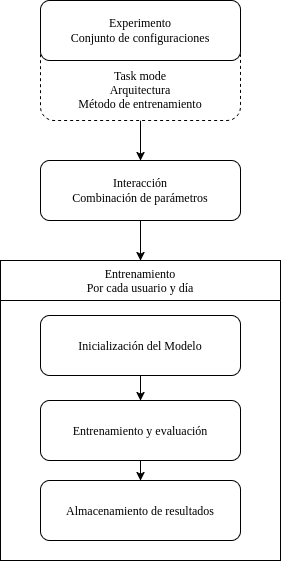
\includegraphics[width=0.45\textwidth]{img/diagrama_pipeline.drawio.png}
    %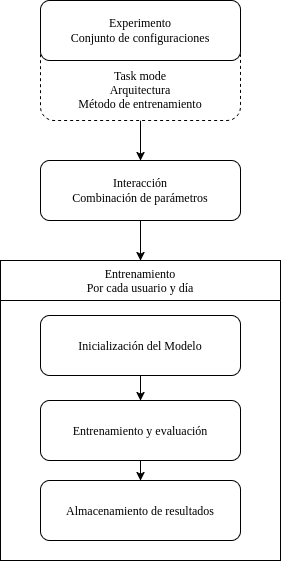
\includegraphics[height=\dimexpr\pagegoal-\pagetotal-\baselineskip\relax,width=\textwidth,keepaspectratio]{img/diagrama_pipeline.drawio.png}
    \caption{Pipeline experimental}
    \label{fig:pipeline_general}
\end{figure}

\subsection{Materiales}
\subsubsection{Hardware}

Para ejecutar los distintos entrenamientos se ha utilizado un ordenador con las siguientes características:

\begin{itemize}
    \item \textbf{CPU}: Intel Core i9-14900HX
    \item \textbf{RAM}: 31 GiB
    \item \textbf{GPU}: NVIDIA GeForce RTX 4060
    \item \textbf{GPU RAM}: 8 GiB
\end{itemize}

Estas características han resultado suficientes para completar los experimentos planteados sin limitaciones críticas. 
El tiempo medio de entrenamiento por iteración ha sido aproximadamente 40 minutos, dependiendo de la configuración del modelo y de los parámetros de entrenamiento. 

El tiempo total de cómputo se estima mediante:


\begin{equation*}
    \text{Tiempo total (h)} = \frac{N_{\text{iteraciones}} \times t_{\text{iteración}}}{60}
\end{equation*} 

Donde $N_{\text{iteraciones}} = 1917$ y $t_{\text{iteración}} = 40 \text{minutos}$, resultando en un tiempo total aproximado de 766.8 horas ($\approx 31 \text{días}$).

El uso de hardware con mayores prestaciones permitiría reducir significativamente el tiempo total de entrenamiento y facilitar la realización de un mayor número de experimentos.

\subsubsection{Sofware}

Para el desarrollo del proyecto se ha utilizado una infraestructura basada en herramientas ampliamente empleadas en el ámbito del aprendizaje automático y la ingeniería de software.

Como lenguaje de programación principal se ha utilizado Python\footnote{https://www.python.org/}, debido a su amplio ecosistema de librerías científicas y de aprendizaje automático, así como su facilidad de integración con frameworks de alto nivel.

Para la construcción y entrenamiento de los modelos se han utilizado TensorFlow\footnote{https://www.tensorflow.org/} y Keras\footnote{https://keras.io/}, frameworks de aprendizaje profundo que permiten definir, entrenar y evaluar redes neuronales de forma eficiente. Keras se ha empleado como interfaz de alto nivel sobre TensorFlow, facilitando la experimentación rápida con distintas arquitecturas.

Durante las etapas iniciales del proyecto se empleó Jupyter Notebook\footnote{https://jupyter.org/} para la realización de pruebas exploratorias y la visualización preliminar de resultados. Sin embargo, su uso fue descartado en fases posteriores debido a la dificultad para mantener una estructura de código modular y escalable en experimentos de mayor complejidad.

Posteriormente, se adoptó Visual Studio Code\footnote{https://code.visualstudio.com/} como entorno de desarrollo principal, debido a su capacidad para gestionar múltiples tipos de archivos y su integración con herramientas de desarrollo. Se utilizaron extensiones específicas para Python, Jupyter y GitHub, permitiendo un flujo de trabajo unificado.

Como sistema de control de versiones se ha utilizado GitHub\footnote{https://github.com/}, que facilita la gestión del código, el seguimiento de cambios y la colaboración con el tutor del proyecto. Además, permite la sincronización del repositorio entre distintos dispositivos de forma eficiente.

Para la visualización de resultados se ha utilizado Vega-Altair\footnote{https://altair-viz.github.io/}, una librería de visualización estadística declarativa enfocada en la simplicidad, eficiencia y legibilidad. A diferencia de enfoques imperativos como Matplotlib, Altair permite definir visualizaciones de forma estructurada y reproducible, enfocándose en lo que se quiere observar en lugar de en los detalles de la implementación. Esto conduce a un código más limpio y legible\cite{geeks_altair_2025}.

Como gestor de base de datos se ha utilizado DuckDB\footnote{https://duckdb.org/}, un sistema de bases de datos analítico embebido que permite realizar consultas SQL de forma eficiente directamente sobre archivos locales. Su integración con Python y su alto rendimiento lo hacen especialmente adecuado para el procesamiento de grandes volúmenes de resultados experimentales\cite{duckdb_2026}.

Todas estas herramientas han sido integradas en un flujo de trabajo unificado orientado a la ejecución reproducible de experimentos.

\subsection{Estructura Dataset}

El dataset utilizado se compone por dos ficheros de labels y dos de datos de entrenamiento. Los labels contienen la intención de movimiento de cada canal de EEG, mientras que los datos contienen las lecturas de cada canal de EEG.

Estos ficheros están separados por la tarea a analizar, de esta forma tenemos los cuatro ficheros:

\begin{center}
    \begin{tabular}{|c|c|c|}
        \hline
         & \textbf{Labels} & \textbf{Training} \\ \hline
        \textbf{Static} &\texttt{labels\_static\_data.mat} & \texttt{training\_static\_data.mat} \\ \hline
        \textbf{Motion} &\texttt{labels\_motion\_data.mat} & \texttt{training\_motion\_data.mat} \\ \hline
    \end{tabular}
\end{center}

%% también puedo ponerlo así
\begin{itemize}
    \item \texttt{labels\_static\_data.mat}
    \item \texttt{training\_static\_data.mat}
    \item \texttt{labels\_motion\_data.mat}
    \item \texttt{training\_motion\_data.mat}
\end{itemize}

Los ficheros contienen la siguiente estructura de datos:
Los labels tienen la forma (15400, 1), mientras que los datos tienen la forma (15400, 27, 400).
Los ficheros de labels contienen una matriz con el numero de ventanas y una columna con la intención de movimiento
Los ficheros de training contienen una matriz de tamaño $N \times C \times S$, donde $N$ es el número de ventanas, $C$ es el número de canales y $S$ es el número de muestras. En el caso de este experimento $N = 15400$ $C = 27$ y $S = 400$. Las muestras son obtenidas durante 2 segundos a 200hz

%% ESTA PARTE ESTÁ Sacada del paper original de donde se sacan los datos
The 27 channels selected for acquisition were: F3, FZ, FC1, FCZ, C1, CZ, CP1, CPZ, FC5, FC3, C5, C3, CP5, CP3, P3, PZ, F4, FC2, FC4, FC6, C2, C4, CP2, CP4, C6, CP6, P4. They were placed following the 10-10 international system.
Four electrodes were located next to the eyes to record electrooculography (EOG) and ground and reference electrodes were located on the right and left ear lobes, respectively. Each channel signal was amplified with BrainVision BrainAmp amplifier. 

%NOSE COMO PONER ESTO:
Se tienen los datos de 5 usuarios, con 5 días cada uno, 11 trials por día, cada día, 56 ventanas por trial. Por lo tanto, se tienen 5 x 5 x 11 x 56 = 15400 ventanas.

Cada trial corresponde a una secuencia de dos tareas mentales, relajación e imaginación de la marcha, que se repite en intervalos de 14 ventanas temporales (0.5s x ventana = 0.7s) de relajación, 28 de imaginación de la marcha (0.5s x ventana = 1.4s) y finalmente otras 14 de relajación. 
Se cuenta con un periodo inicial de duración aleatoria en la cual se le pedía al sujeto realizar una tarea mental compleja, diferente a la imaginación motora. Este periodo se utiliza para eliminar ruidos en la señal EEG y se ha eliminado del dataset final.

Un esquema de las ventanas se puede ver en la figura \ref{fig:ventanas}.

\begin{figure}[H]
    \centering
    
\includegraphics[width=0.8\textwidth]{ventanas.png}
    \caption{Esquema de las ventanas}
    \label{fig:ventanas}
\end{figure}

Los labels y los datos están relacionados a nivel de ventana, utilizando un fichero auxiliar vector_tasks_training.mat.

\subsubsection{Preprocesamiento de datos}

Los datos han sido procesados previamente en otro estudio.
Para este trabajo, se modificaron los arrays para que tuvieran 6 dimensiones (input) y 5 dimensiones (labels):
input_6d = input_data.reshape(N_USERS,N_DAYS,N_TRIALS,N_WINDOWS,N_CHANNELS,N_SAMPLES)
labels_6d = labels_data.reshape(N_USERS,N_DAYS,N_TRIALS,N_WINDOWS,1)

La separación entre los datos de entrenamiento y testeo se ha hecho en un 70\% de entrenamiento y 30\% de testeo y se aplica al nivel de trial. Esta separación se ha hecho para cada entrenamiento del modelo y se toma en cuenta el usuario y día de cada uno. No se ha hecho de manera aleatoria, sino que se han utilizado para testeo empezando por el final de la lista de trials. 

La razón de esta decisión es que en los primeros trials el sujeto suele presentar un menor control sobre su imaginación motora. %esta frase no me gusta ni un pelooooooo

Más allá de estos preprocesamientos, no se ha hecho nada más

la Pipeline
qué hace tu sistema de principio a fin

Ejemplo:

    entrada: EEG

    procesamiento

    modelo

    salida: predicción


\subsection{Modelos utilizados}
Aquí metes:

\subsubsection{EEGNet}
\subsubsection{DeepConvNet}
\subsubsection{ShallowConvNet} (si lo usas)

Para cada uno:

    breve descripción (2–3 líneas)

    por qué lo eliges

NO pongas la arquitectura entera en detalle aquí (eso es más de anexos si acaso)

\subsection{Metodología experimental}

Aquí es donde entra todo tu proyecto de verdad.
\subsubsection{Variables del estudio}

Muy importante estructurarlo así:

    Arquitectura del modelo

    Método de entrenamiento:

        same-day

        acumulativo

        fine-tuning

    Tarea:

        static / motion

    Usuario

\subsubsection{Estrategia de entrenamiento}\label{sec:metodos_entrenamiento}

    epochs

    batch size

    callbacks:

        early stopping

        reduce LR

    función de pérdida

    métrica (accuracy)

No te líes demasiado, pero deja claro cómo entrenas



\subsubsection{Evaluación}

MUY importante:

    validación cruzada

    pseudo-online

explica qué significa pseudo-online (aunque sea breve)



\subsection{Infraestructura Experimental}

Aquí metes tu microframework (esto es TU aporte técnico fuerte)

sistema para ejecutar múltiples experimentos
gestión de parámetros
almacenamiento de resultados (DuckDB)
automatización

Esto es diferencial → véndelo bien


Se ha programado un microframework para el desarrollo de experimentos de Machine Learning.

Como se ha comentado en el apartado \ref{sec:}, se ha realizado la comparación de tres modelos de redes neuronales convolucionales para la clasificación de la intención de caminar o detenerse con un exoesqueleto. Se ha utilizado un dataset de EEG con 27 canales, obtenido de una muestra de un estudio previo XXXXXX. Los parametros a comparar son la arquitectura de la red, el metodo de entrenamiento, la tarea a predecir y la variabilidad entre usuarios.

Al necesitarse de cientos de ejecuciones para obtener todos los datos necesarios, durante las etapas iniciales se tomó la decisión de enfocar el proyecto de manera horizontal, preparando una base de ejecución sobre la cual modificar facilmente todo lo necesario para cada ejecución y permitiendo ejecutar multiples experimentos de manera secuencial.

(((((((Aquí no sé si ir diicendo TOOOOODo lo que he ido poniendo en el código. Puedo ir siguiendo el timeline de Github y hacer un resumen de los commits))))))))


\subsubsection{Diseño de experimentos}

Aquí explicas cómo organizaste TODO

combinaciones de parámetros
nº de ejecuciones
cómo comparas resultados

Esto conecta directamente con Results luego

%%%%%%%%%%%%%%%%%%% - Resultados y discusion - %%%%%%%%%%%%%%%%%%

\section{Resultados y Discusión} \label{sec:resultados}

Los resultados obtenidos durante la experimentación se han almacenado en una base de datos DuckDB, tal y como se describió en la Sección \ref{sec:infraestructura_exp}. Las tablas generadas contienen, para cada ejecución realizada, tanto los metadatos asociados al entrenamiento como las métricas obtenidas durante su evaluación.

Con el objetivo de reducir la influencia de posibles valores atípicos (\textit{outliers}) sobre el análisis estadístico, se han creado vistas derivadas de cada tabla en las que se eliminan aquellos registros cuyos valores de \textit{accuracy} se encuentran fuera de un intervalo de tres desviaciones estándar respecto a la media. Este procedimiento, basado en el método \textit{Z-Score} \cite{venkataanusha_DetectingOutliers2019}, se define como:

\[
z = \frac{x - \mu}{\sigma}
\]

donde \(x\) representa el valor analizado, \(\mu\) la media de la distribución y \(\sigma\) la desviación estándar. De esta forma, se consideran valores atípicos aquellos que cumplen:

\[
|z| > 3
\]

Además, también se han eliminado aquellos registros correspondientes a entrenamientos incompletos o interrumpidos, con el fin de garantizar la consistencia de los resultados analizados.

Tras aplicar este proceso de filtrado, el número total de registros válidos quedó reducido de la siguiente manera:

\begin{itemize}
    \item Tabla de entrenamientos: de 1917 registros originales se eliminaron 105, obteniéndose un total de 1812 registros válidos.
    
    \item Tabla de trials: de 5751 registros originales se eliminaron 515, obteniéndose un total de 5246 registros válidos.
    
    \item Tabla de clases: de 15336 registros originales se eliminaron 3331, obteniéndose un total de 12605 registros válidos.
\end{itemize}

En esta sección se presentarán estos resultados, los cuales se discutirán y analizarán siguiendo la siguiente metodología:

Primero se analizarán los resultados obtenidos por cada modelo en función de la tarea 

\subsection{Tarea Estática} \label{sec:tareaestatica} 

\subsubsection{Comparación de Global}

\begin{figure}[H]
    \centering
    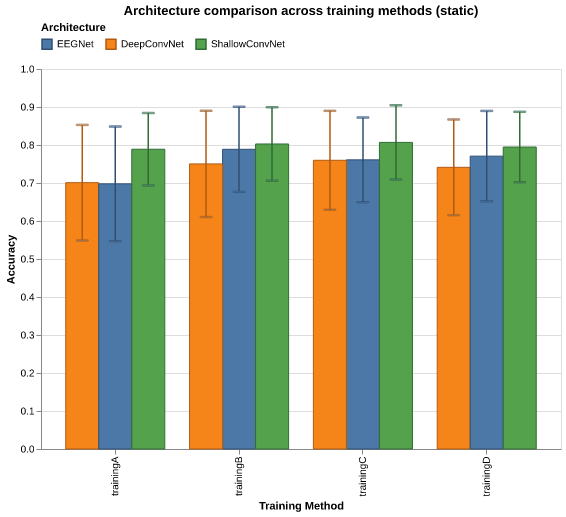
\includegraphics[width=0.90\textwidth]{img/resultados/architecture_training_comparison_clean_static.png}
    %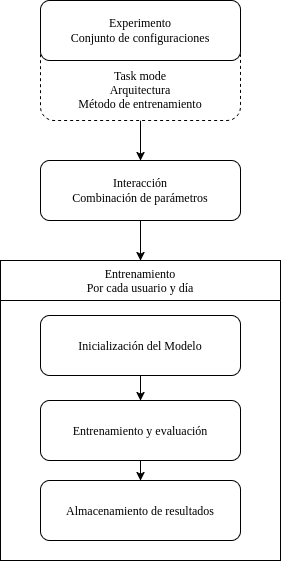
\includegraphics[height=\dimexpr\pagegoal-\pagetotal-\baselineskip\relax,width=\textwidth,keepaspectratio]{img/diagrama_pipeline.drawio.png}
    \caption{Comparación general de las distintas arquitecturas y métodos de entrenamiento en la tarea estática}
    \label{fig:architecture_training_comparison_clean_static}
\end{figure}


Me da igual todo, solo me centro en los modelos. hago avg y std con los metodos y los usuarios 

\subsubsection{Comparación de Método de Entrenamiento}
Me da igual todo, solo me centro en los metodos. hago avg y std con los modelos y los usuarios 

\subsubsection{Variabilidad Entre Usuarios}

\begin{figure}[H]
    \centering
    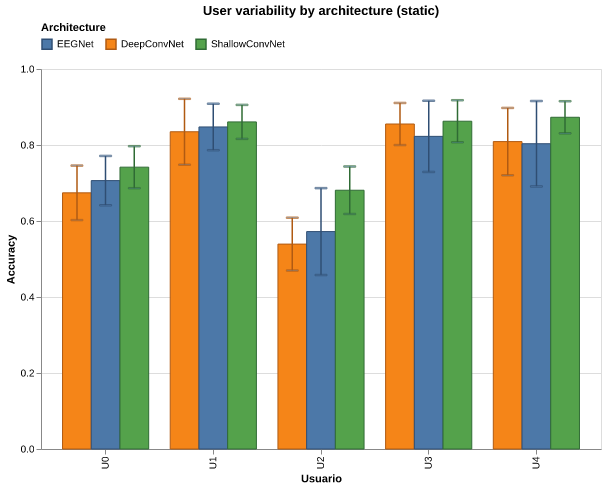
\includegraphics[width=0.90\textwidth]{img/resultados/user_variability_by_model_static.png}
    %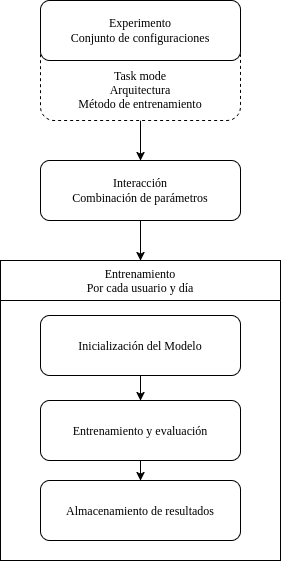
\includegraphics[height=\dimexpr\pagegoal-\pagetotal-\baselineskip\relax,width=\textwidth,keepaspectratio]{img/diagrama_pipeline.drawio.png}
    \caption{Variabilidad entre usuarios en la tarea estática}
    \label{fig:user_variability_by_model_static}
\end{figure}

\subsubsection{Mejor Configuración}

\begin{figure}[H]
    \centering
    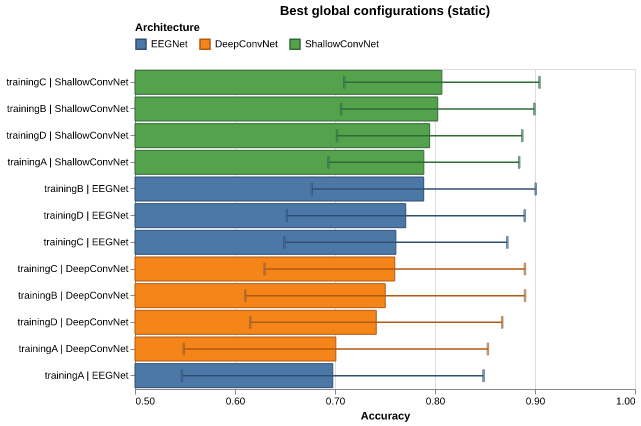
\includegraphics[width=1\textwidth]{img/resultados/best_global_configurations_static.png}
    %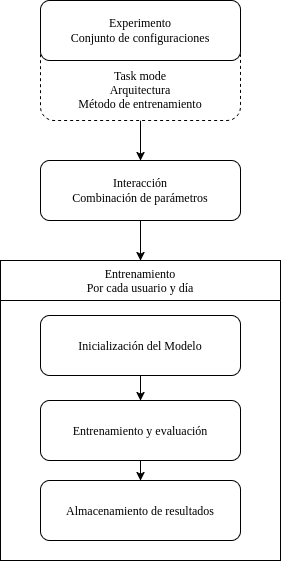
\includegraphics[height=\dimexpr\pagegoal-\pagetotal-\baselineskip\relax,width=\textwidth,keepaspectratio]{img/diagrama_pipeline.drawio.png}
    \caption{Mejores configuraciones globales en la tarea estática}
    \label{fig:best_global_configurations_static}
\end{figure}

\subsection{Tarea Movimiento} \label{sec:tareamovimiento} 
mismo esquema 

\subsubsection{Comparación de Global}

\begin{figure}[H]
    \centering
    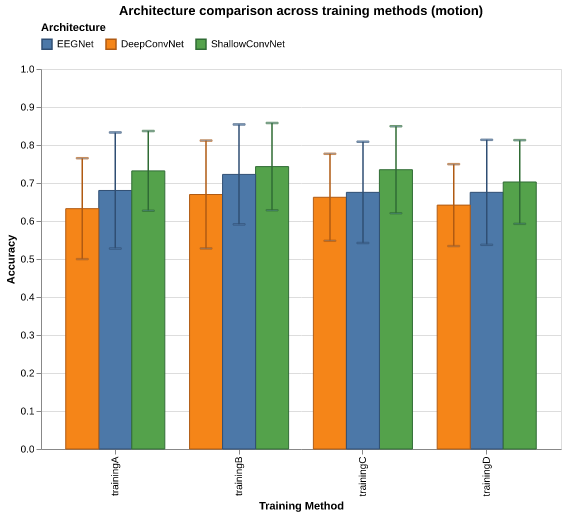
\includegraphics[width=0.90\textwidth]{img/resultados/architecture_training_comparison_clean_motion.png}
    %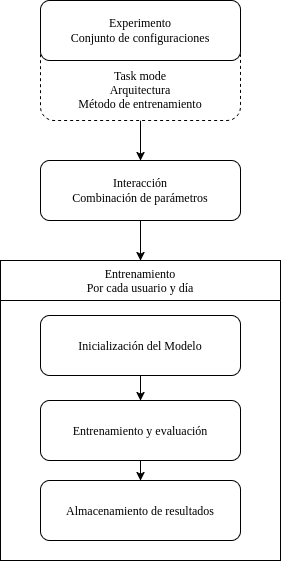
\includegraphics[height=\dimexpr\pagegoal-\pagetotal-\baselineskip\relax,width=\textwidth,keepaspectratio]{img/diagrama_pipeline.drawio.png}
    \caption{Comparación general de las distintas arquitecturas y métodos de entrenamiento en la tarea de movimiento}
    \label{fig:architecture_training_comparison_clean_motion}
\end{figure}


\subsubsection{Comparación de Método de Entrenamiento}
\subsubsection{Variabilidad Entre Usuarios}
\begin{figure}[H]
    \centering
    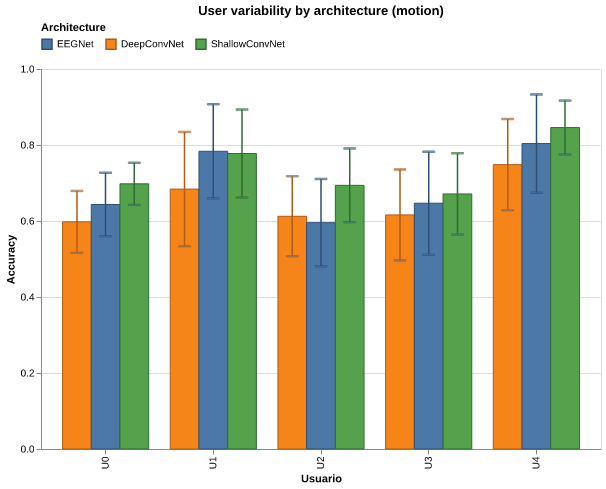
\includegraphics[width=0.90\textwidth]{img/resultados/user_variability_by_model_motion.png}
    %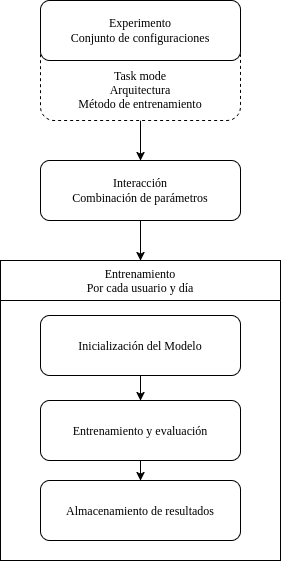
\includegraphics[height=\dimexpr\pagegoal-\pagetotal-\baselineskip\relax,width=\textwidth,keepaspectratio]{img/diagrama_pipeline.drawio.png}
    \caption{Variabilidad entre usuarios en la tarea de movimiento}
    \label{fig:user_variability_by_model_motion}
\end{figure}

\subsubsection{Mejor Configuración}

\begin{figure}[H]
    \centering
    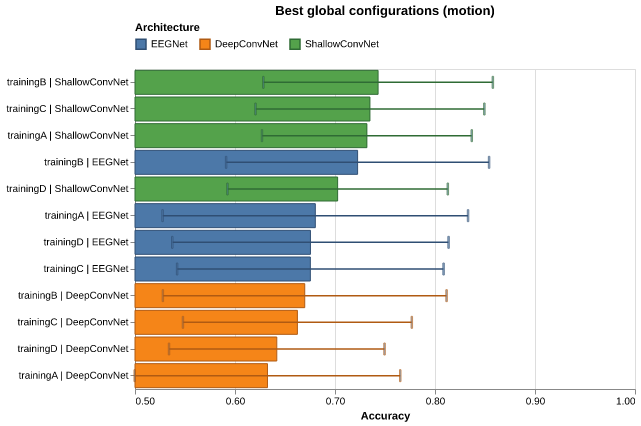
\includegraphics[width=1\textwidth]{img/resultados/best_global_configurations_motion.png}
    %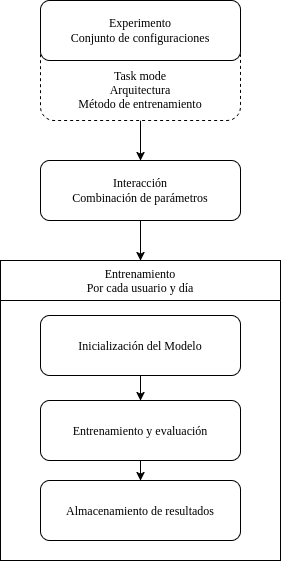
\includegraphics[height=\dimexpr\pagegoal-\pagetotal-\baselineskip\relax,width=\textwidth,keepaspectratio]{img/diagrama_pipeline.drawio.png}
    \caption{Mejores configuraciones globales en la tarea de movimiento}
    \label{fig:best_global_configurations_motion}
\end{figure}

\subsection{Comparación entre tareas}


\begin{figure}[H]
    \centering
    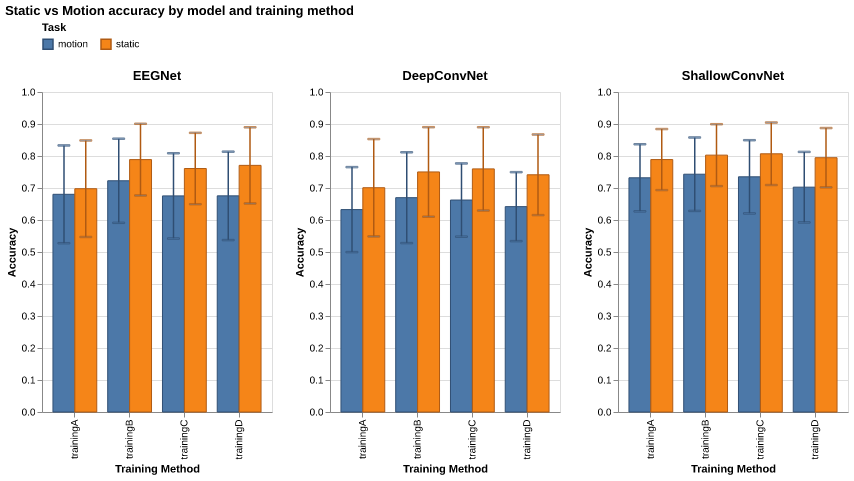
\includegraphics[width=1\textwidth]{img/resultados/static_vs_motion_accuracy.png}
    %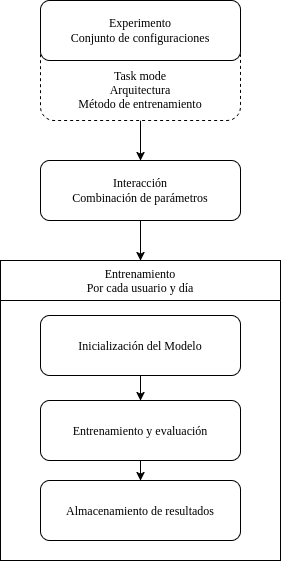
\includegraphics[height=\dimexpr\pagegoal-\pagetotal-\baselineskip\relax,width=\textwidth,keepaspectratio]{img/diagrama_pipeline.drawio.png}
    \caption{Comparación de la precisión entre la tarea estática y la de movimiento}
    \label{fig:static_vs_motion_accuracy}
\end{figure}



%%%%%%%%%%%%%%%%%%% - Conclusiones - %%%%%%%%%%%%%%%%%%

\section{Conclusiones} \label{sec:conclusiones}


En este trabajo se ha estudiado el rendimiento de tres arquitecturas de redes neuronales convolucionales, \textit{EEGNet}, \textit{DeepConvNet} y \textit{ShallowConvNet}, para la clasificación de señales EEG asociadas a las tareas estática y de movimiento durante el uso de un exoesqueleto. Asimismo, se han comparado cuatro estrategias de entrenamiento: \textit{Intra-Sesión}, \textit{Inter-Sesión}, \textit{Inter-Usuarios} y \textit{Continuo}.

Hay estudios que señalan que el rendimiento de los modelos de DeepLearning para \acrshort{eeg} depende en gran medida del conjunto de datos, del paradigma experimental y de la estrategia de entrenamiento utilizada. Por este motivo es difícil establecer una arquitectura o un método de entrenamiento que sea superior en todas las aplicaciones, sino que debe evaluarse bajo las condiciones concretas de cada problema \cite{kollod_DeepComparisons2023}.

Los resultados obtenidos muestran, de manera general, que la arquitectura, la tarea analizada y el usuario tienen una mayor influencia sobre el rendimiento que el método de entrenamiento. Aunque se observan diferencias entre las estrategias de entrenamiento, estas no se mantienen de forma consistente entre todas las arquitecturas, tareas y participantes.

\subsection{Influencia de la arquitectura}

La arquitectura \textit{ShallowConvNet} presenta el mejor rendimiento global, con una precisión media aproximada del 76.6\%. \textit{EEGNet} obtiene un resultado intermedio, cercano al 71.4\%, mientras que \textit{DeepConvNet} alcanza la precisión media más baja, con aproximadamente un 69.4\%.

La superioridad de \textit{ShallowConvNet} se mantiene entre las dos tareas y los diferentes métodos de entrenamiento. Además, esta arquitectura muestra un comportamiento relativamente estable frente a los cambios de configuración, aunque presenta una variabilidad considerable entre usuarios.

Por su parte, \textit{EEGNet} obtiene resultados intermedios en la mayoría de las configuraciones. El estar orientado a diferentes paradigmas BCI puede favorecer su capacidad de generalización, aunque la escasez del conjunto de datos utilizado en este estudio puede hacer que esta arquitectura no alcance el rendimiento esperado.

\textit{DeepConvNet} presenta generalmente los peores resultados y una mayor reducción de precisión en la tarea de movimiento. Una posible explicación es que su mayor número de parámetros requiera una mayor cantidad de datos para aprender y generalizar a nuevas observaciones. Es posible que esta arquitectura no haya podido obtener el rendimiento esperado debido al número limitado de participantes y sesiones disponibles,

Sin embargo, también hay que tener en cuenta que se ha utilizado una configuración de hiperparámetros común en todos los experimentos. Aunque esta decisión permite reducir la complejidad del estudio, puede favorecer a determinados modelos, ya que cada arquitectura podría requerir una configuración específica para obtener su rendimiento óptimo.

A falta de una búsqueda de parámetros exhaustiva, los resultados indican que la elección de la arquitectura tiene una influencia más evidente que la elección del método de entrenamiento.

\subsection{Influencia de la tarea}

La tarea estática alcanza una precisión media global aproximada del 76.0\%, mientras que la tarea de movimiento obtiene un valor cercano al 69.1\%. Esto supone una diferencia media de aproximadamente siete puntos porcentuales a favor de la tarea estática.

La mayoría de configuraciones de arquitecturas, métodos de entrenamiento y usuarios analizados presentan una mayor precisión en la tarea estática. Por tanto, los resultados indican que la tarea de movimiento presenta una mayor dificultad de generalización.

Una posible explicación es que los patrones EEG asociados a la tarea de movimiento sean más variables o menos diferenciables que los relacionados con la tarea estática. Los posibles factores que pueden contribuir a esta diferencia son: el cambio en la concentración de los participantes, la presencia de artefactos o las características concretas del protocolo de adquisición.

Sin embargo, los resultados obtenidos no permiten determinar cuál de estos factores es el responsable de la diferencia observada. Para ello sería necesario realizar un análisis más específico de las señales y de las condiciones experimentales de cada tarea.

\subsection{Variabilidad entre usuarios}

El propio usuario se presenta como uno de los factores con mayor influencia sobre los resultados. La desviación estándar de las precisiones medias de los participantes alcanza los 9.15 puntos porcentuales, mientras que el rango de medias globales va desde aproximadamente un 61.6\% para el \textbf{usuario 2} hasta un 81.3\% para el \textbf{usuario 4}, lo que supone una diferencia cercana a 20 puntos porcentuales entre ambos. Esta dispersión es superior a la observada entre los métodos de entrenamiento y sugiere una importante dependencia del rendimiento respecto al participante.

Además, el comportamiento de los usuarios no presenta una tendencia general. Por ejemplo, el \textbf{usuario 1} obtiene los mejores resultados en la tarea estática, mientras que el \textbf{usuario 4} presenta el mejor rendimiento en la tarea de movimiento. Aunque, en general, la precisión de la tarea estática supera a la de movimiento en aproximadamente 7 puntos, esta diferencia no se observa de la misma forma en todos los participantes. El \textbf{usuario 2}, por ejemplo, mejora 3 puntos porcentuales en la tarea de movimiento, mientras que el \textbf{usuario 3} experimenta una reducción cercana a 20 puntos.

Estas diferencias pueden estar relacionadas con la variabilidad fisiológica de las señales EEG, la calidad del registro, la colocación de los electrodos, la capacidad de concentración o la forma en que cada participante ejecuta las tareas. El hecho de que el orden relativo de los usuarios cambie entre tareas indica que no todos los participantes se ven afectados de la misma manera por la complejidad de la tarea.

En conjunto, los resultados muestran una elevada variabilidad inter-sujeto.


\subsection{Influencia de los métodos de entrenamiento}

El método \textit{Inter-Sesión} obtiene la mayor precisión media global, con aproximadamente un 74.8\%. Después va el entrenamiento \textit{Inter-Usuarios}, con un 72.9\%, seguido del entrenamiento \textit{Continuo}, con un 71.4\%, y del entrenamiento \textit{Intra-Sesión}, con un 70.4\%.

El menor rendimiento del método \textit{Intra-Sesión} era de esperar, ya que al utilizar datos de un único día y usuario, el modelo dispone de menos ejemplos para aprender y generalizar. Además puede presentar una mayor dependencia de las características particulares de esa sesión.

El método \textit{Inter-Sesión} puede aprovechar información de sesiones anteriores del mismo usuario, lo que permite aumentar la cantidad de datos de entrenamiento. Además, al centrarse en un único participante, el modelo no se enfrenta a la variabilidad asociada a otros usuarios. Esto podría explicar su mayor precisión media y su menor desviación.

Los entrenamientos \textit{Inter-Usuarios} y \textit{Continuo} no presentan una mejora claramente diferenciada respecto al entrenamiento \textit{Intra-Sesión}. Esto quiere decir que el uso de un modelo inicial entrenado con otros usuarios no garantiza un aumento de la precisión tras su adaptación al usuario objetivo.

Una posible explicación es que, las características compartidas entre participantes sean limitadas y que el conocimiento adquirido con otros usuarios no pueda transferirse directamente. También es posible que, durante la adaptación individual, el modelo modifique parte de los pesos generales aprendidos sin disponer todavía de suficientes datos del usuario objetivo, perdiendo así información relevante. Queda por determinar si una modificación en el modelo general o en el proceso de \textit{fine-tuning} puede mejorar el rendimiento del modelo específico.

En cualquier caso, los resultados no permiten establecer un método de entrenamiento claramente superior. Aunque \textit{Inter-Sesión} presenta el mejor rendimiento medio, no presenta la misma mejora en todas las arquitecturas, tareas y usuarios. Esto no implica que los métodos sean equivalentes. Los resultados pueden indicar que sus diferencias son menores que las producidas por los otros factores.

\subsection{Conclusión general}

En general, se puede concluir que \textit{ShallowConvNet} es la arquitectura más adecuada para este conjunto de datos, al presentar la mayor precisión media y un comportamiento comparativamente estable entre tareas y métodos de entrenamiento.

También se observa una diferencia clara entre las dos tareas estudiadas. La tarea estática obtiene mejores resultados que la tarea de movimiento de manera consistente, aunque no se puede obtener una razón concreta de esta diferencia a partir de los resultados obtenidos.

En cuanto a las estrategias de entrenamiento, \textit{Inter-Sesión} presenta los mejores resultados medios, pero la mejora respecto a los demás métodos no es consistente. Los métodos que incorporan información de otros usuarios no consiguen una ventaja suficientemente grande como para justificar la mayor complejidad en su proceso de entrenamiento.

En las condiciones evaluadas, aumentar la complejidad de la estrategia de entrenamiento equivale necesariamente a una mejora proporcional de la precisión. La arquitectura seleccionada y las características particulares del usuario y de la tarea parecen ser factores más determinantes.

Finalmente, la elevada variabilidad entre usuarios sugiere que la capacidad de generalización de los modelos está extremadamente condicionada por las características individuales de las señales EEG. Esto puede dificultar la elección de una configuración óptima de arquitectura y método de entrenamiento que sea válida para todos los participantes.

  {
    \begin{comment}


    Este apartado introductorio faltaría rellenarlo con las conclusiones obtenidas a partir de los resultados del capítulo anterior.




    ShallowConvNet suele ser el mejor.

    DeepConvNet normalmente el peor.

    Static funciona mejor que Motion.

    Hay bastante dependencia del usuario.

    Inter-Sesión e Inter-Users mejoran ligeramente respecto a Intra.

    Continuous no supone una mejora espectacular.

    Me queda realmente poco, comentar los resultados y las conclusiones. Viendo las gráficas se queda algo así:

    ShallowConvNet suele ser el mejor. (global Avg= 0.76)
    EEGNet Suele mantenerse en el medio (global Avg = 0.71)
    DeepConvNet normalmente el peor. (global Avg = 0.69)
    model\_name         avg\_acc1
    varchar            double

    ShallowConvNet  0.7662446249402762
    DeepConvNet     0.6937626027609743
    EEGNet          0.7137599206349203

    Static funciona mejor que Motion.
    task\_mode       avg\_acc1
    varchar         double

    motion     0.6906362007168463
    static     0.7598059064895796


    Hay bastante dependencia del usuario.
    user        avg\_acc1
    int64        double

    0  0.6762566137566141
    1  0.7917231766124173
    2   0.615861618798956
    3  0.7458137100994237
    4  0.8133346823148518


    Inter-Sesión e Inter-Users mejoran ligeramente respecto a Intra.

    training\_method       avg\_acc1
    varchar            double

    trainingA        0.7044462481962481  -> intrasesión
    trainingB        0.7478039759593151  -> inter sesiones
    trainingC        0.7294351951306842  -> inter users
    trainingD         0.713930348258706  -> continuous



    Continuous no supone una mejora espectacular.

    Solo habría que argumentarlos o dar una hipótesis.
    En el caso de los métodos de las arquitecturas se pueden argumentar ligeramente con estas frases:
    EEGNet, es agnóstico al paradigma BCI, por lo que sus resultados pueden ser buenos, pero al no estar optimizada para MRCP puede quedarse atrás.

    DeepConvNet y ShallowConvNet sí fueron entrenados y diseñados con datos MRCP (l1 = Hand Left, l2 = Hand Right,  l3 = Feet, l4 = Rest)
    En el paper original DeepConvNet obtiene ligeramente peores resultados que ShallowConvNet en varios datasets (-5\%). La diferencia observada en este estudio (-10\%) puede atribuirse a que DeepConvNet, al tener un mayor número de parámetros entrenables, requiere a su vez más cantidad de datos para poder generalizar correctamnete. Debido a la limitada cantidad de datos utilizados en este estudio (5 usuarios y 5 sesiones), el rendimiento de DeepConvNet suele ser peor.

    Las tereas:
    motion suele tener más ``ruido mental'', suele ser más dificil concentrarse moverse, y suele ser mas complejo diferenciarlo en las señales.
    static en cambio suele sér más sencillo.

    Los entrenamientos:
    Se puede estipular que intra-sesion tiene muy pocos datos y que no es capaz de generalizar.
    Inter-sesiónes, tiene más datos que intra sesión. Además aprende de manera iterativa, al utilizar los datos de las sesiones anteriores, los modelos finales aprenden correctamente los patrones que se han visto en las sesiones anteriores, además el centrarse en un unico usuario no se enfrenta al problema de la variabilidad entre ellos.
    Continious y inter Users: se puede estipular que el añadir los datos de todos los usuarios y todas las sesiones puede hacer que aprenda correctamente datos globales, pero que al entrenar individualmente con los datos de cada usuario pierda el conocimiento que aprendió con los datos de otros usuarios.


    Esta ausencia de una ventaja sistemática no implica que los métodos produzcan resultados equivalentes, sino que, con los datos disponibles, sus diferencias quedan parcialmente ocultas por otros factores de mayor influencia, como la arquitectura seleccionada y la variabilidad entre sujetos.

    En conjunto, la elevada variabilidad entre los usuarios  puede dificultar la mejora en los resultados por los métodos de entrenamiento. Las diferencias fisiológicas, la calidad de las señales registradas y la capacidad de cada participante para realizar la tarea pueden producir variaciones superiores al efecto del propio método.

    Por tanto, para la tarea estática, la arquitectura utilizada tiene un efecto más visible sobre la precisión que el método de entrenamiento.

    Esta modificación del orden relativo de los usuarios sugiere que la dificultad de la tarea depende también de las características particulares de cada sujeto.

    Las diferencias entre usuarios vuelven a superar, en numerosos casos, las observadas entre métodos de entrenamiento. Este comportamiento sugiere que la capacidad de generalización de los modelos está condicionada por la variabilidad de las señales EEG individuales, especialmente en la tarea de movimiento.

    No obstante, a partir de este análisis descriptivo no puede determinarse por sí solo si esta diferencia se debe a una mayor complejidad fisiológica de la tarea, a las características del protocolo experimental o a diferencias en la calidad de las señales registradas.


    Por tanto, los resultados obtenidos no respaldan la existencia de un método de entrenamiento universalmente superior. La estrategia utilizada parece tener un efecto secundario frente a otros factores, especialmente la arquitectura, la tarea y la identidad del usuario. También es posible que el reducido número de sujetos y sesiones limite la capacidad del análisis para detectar diferencias moderadas entre métodos.

    Esta falta de diferencias constituye en sí misma un resultado relevante: dentro de las condiciones experimentales estudiadas, aumentar la complejidad del procedimiento de entrenamiento no se traduce necesariamente en una mejora proporcional del rendimiento.

    Los métodos de entrenamiento
    \end{comment}
  }

\subsection{Trabajos futuros}

\subsubsection{Maquina de estados finitos}

Una posible línea de trabajo futuro consiste en integrar dos modelos distintos dentro de un mismo sistema de control, con el objetivo de aprovechar las dos tareas de imaginación motora para construir una \acrshort{bci} de bucle cerrado basada en una máquina de estados finitos. Este enfoque permitiría controlar de forma independiente el comportamiento del exoesqueleto y proporcionar al usuario un mayor grado de autonomía durante la interacción.

En este planteamiento, el sistema comenzaría en un estado de \textbf{parada}, en el que el exoesqueleto permanecería inmóvil mientras un modelo entrenado sobre la tarea estática (\textit{Modelo de Inicio de la Marcha}) monitoriza continuamente la actividad cerebral del usuario. Cuando dicho modelo detectase una intención de inicio de la marcha, el sistema realizaría una transición al estado de \textbf{movimiento}.

Durante este segundo estado, el exoesqueleto ejecutaría la marcha asistida mientras un modelo entrenado sobre la tarea en movimiento (\textit{Modelo de Detención}) analiza la señal EEG en busca de una intención de parada. Una vez detectada esta intención, el sistema regresaría al estado de \textbf{parada}, completando así el ciclo de control.

Con el objetivo de reducir la probabilidad de falsos positivos, las predicciones de ambos modelos podrían combinarse mediante una estrategia basada en una media ponderada. De esta forma, aunque cada estado disponga de un clasificador principal, la decisión final tendría en cuenta la información proporcionada por ambos modelos, aumentando potencialmente la robustez del sistema frente a errores de clasificación.

La Figura \ref{fig:diagrama_estados} muestra una representación conceptual de esta máquina de estados finitos y de las transiciones asociadas a cada uno de los modelos de clasificación.

\begin{figure}[htbp]
  \centering
  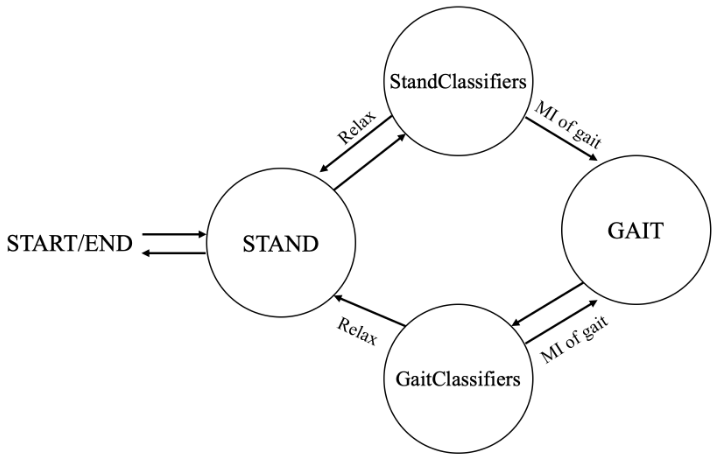
\includegraphics[width=0.90\textwidth]{img/diagrama_estados_ferrero.png}
  %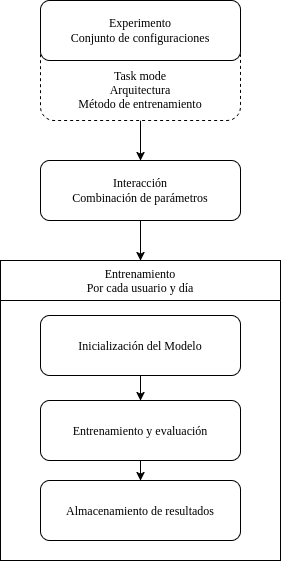
\includegraphics[height=\dimexpr\pagegoal-\pagetotal-\baselineskip\relax,width=\textwidth,keepaspectratio]{img/diagrama_pipeline.drawio.png}
  \caption{Ejemplo de arquitectura de control basada en una máquina de estados finitos para sistemas BCI. Tomado de \cite{ferrero_BMIBased2021}}
  \label{fig:diagrama_estados}
\end{figure}

Este procedimiento es consistente con diversas propuestas presentes en la literatura, donde el control de sistemas \acrshort{bci} se aborda mediante máquinas de estados finitos donde varios clasificadores de EEG son utilizados para detectar las distintas intenciones del usuario, tales como iniciar, mantener, o finalizar la marcha. En esta línea, Ferrero et al. \parencite{ferrero_BMIBased2021} emplean una arquitectura de control basada en estados para gobernar la marcha de un exoesqueleto, mientras que los mismos autores \parencite{ferrero_BCIBased2021} aplican un enfoque similar al control de una cinta de marcha.

Asimismo, \textcite{choi_DevelopingMotor2020} demostraron la viabilidad de este paradigma en sistemas de control asíncronos para exoesqueletos de miembro inferior, utilizando tres estados funcionales (parada, marcha y sentado) y transiciones activadas mediante imaginación motora.

\subsubsection{Interpretabilidad de los modelos utilizados}

Otra posible línea de investigación consiste en estudiar la interpretabilidad de los modelos entrenados. Tanto \textcite{lawhern_EEGNetCompact2018} como \textcite{schirrmeister_DeepLearning2017} aplicaron estas técnicas para analizar las características aprendidas por las arquitecturas propuestas en sus respectivos trabajos.

Un análisis interpretable permitiría determinar qué componentes de la señal tienen una mayor influencia en la clasificación de cada una de las tareas propuestas. En particular, podría estudiarse la relevancia de los distintos electrodos y regiones espaciales o las de distintas bandas de frecuencia e intervalos temporales.

Este análisis permitiría comprobar si los modelos basan sus decisiones en patrones neurofisiológicos comunes o si, por el contrario, dependen en exceso de artefactos o características particulares del conjunto de datos. Además, la comparación de los patrones aprendidos por \textit{EEGNet}, \textit{DeepConvNet} y \textit{ShallowConvNet} ayudaría a explicar las diferencias de rendimiento observadas entre las arquitecturas.

\subsubsection{Evaluación de la cantidad de datos necesaria}

En los experimentos realizados se utilizaron para el entrenamiento los ocho primeros ensayos de cada día, de un total de once. Esto representa aproximadamente un 73\% de los ensayos disponibles, mientras que los tres restantes se reservaron para la evaluación.

Como trabajo futuro, sería interesante estudiar cómo varía el rendimiento de las arquitecturas al modificar la cantidad de información utilizada durante el entrenamiento. Para ello, podrían entrenarse los modelos utilizando una cantidad diferente de ensayos, pudiendo mantener un conjunto de evaluación común para garantizar que los resultados obtenidos sean comparables.

Este análisis permitiría observar la relación entre la cantidad de datos disponibles y la precisión alcanzada, así como identificar el punto a partir del cual la incorporación de nuevos ensayos no produce grandes mejoras.

También permitiría estimar la cantidad mínima de información necesaria para adaptar un modelo a un nuevo usuario, reduciendo el tiempo de calibración.Esto resulta especialmente relevante para el desarrollo de sistemas \acrshort{bci}, ya que una estrategia capaz de alcanzar un rendimiento adecuado con pocos ensayos facilitaría su adopción por parte de nuevos usuarios y reduciría el tiempo de aprendizaje.

%%%%%%%%%%%%%%%%%%% - Anexos - %%%%%%%%%%%%%%%%%%

%%%%%%%%%%%%%%%%%%% - Contenido de TFG y TFM - %%%%%%%%%%%%%%%%%%

\section{Contenido de TFG y TFM} 

\subsubsection{Estructura y contenidos de un Trabajo de Investigación}
\label{sec:estructuratrabajoinvestigacion}

Un TFG o TFM en la modalidad de Trabajo de Investigación deberá estructurarse en los siguientes apartados:
\begin{enumerate}
    \item \textit{Introducción}: contendrá un estudio del estado actual de la técnica sobre el problema plateado, las alternativas consideradas y los objetivos a conseguir.
    \item \textit{Material y métodos}: se describirán los equipos y materiales utilizados para su realización, la metodología empleada y una descripción completa de los experimentos realizados.
    \item \textit{Resultados y discusión}: se describirán y analizarán los resultados obtenidos siguiendo la metodología propuesta.
    \item \textit{Conclusiones}: en función de los resultados obtenidos, 
    se expondrán las conclusiones de la investigación y se propondrán trabajos futuros.
    \item \textit{Anexos}: tantos como se considere necesario en función de los aspectos concretos que se quieran especificar.
    \item \textit{Bibliografía}: se indicarán todas las referencias bibliográficas utilizadas, ordenadas con código para su cita en la memoria.
\end{enumerate}


%%%%%%%%%%%%%%%%%%%%%%%%%%%%%%%%%%%%%%%%%%%%%%%%%%
 
\section{TABLAS} \label{sec:tablas}

Las tablas se definen en el entorno \texttt{table}. Existen infinidad de posibilidades en cuanto a su formato: omitir o dibujar líneas horizontales y verticales, fusionar columnas y filas, alinear el contenido a la derecha, izquierda o centro, y demás opciones resumidas en \url{https://www.overleaf.com/learn/latex/tables}. Dado que la forma de construir una tabla directamente en código \LaTeX \ está lejos de ser cómoda e intuitiva, quizás lo más recomendable sea acudir a editores de tablas que generan automáticamente el código correspondiente y cuya interfaz es similar a la que puede encontrarse en Excel, como por ejemplo \url{https://www.tablesgenerator.com/}. Un ejemplo sencillo de tabla se muestra a continuación:

\vspace{25pt}

\begin{table}[H]
\centering
\begin{tabular}{|c|c|c|l|}
\hline
$\bm{n}$ & $\bm{a_n}$ & $\bm{a_{n+1}}$ & $\bm{\varphi} \ _{(= a_{n+1}/a_n)}$ \\ \hline\hline
\textbf{1} & 1 & 1 & 1 \\ \hline
\textbf{2} & 1 & 2 & 2 \\ \hline
\textbf{3} & 2 & 3 & 1,5 \\ \hline
\textbf{4} & 3 & 5 & 1,66666667 \\ \hline
\textbf{5} & 5 & 8 & 1,6 \\ \hline
\textbf{6} & 8 & 13 & 1,625 \\ \hline
\textbf{7} & 13 & 21 & 1,61538462 \\ \hline
\textbf{8} & 21 & 34 & 1,61904762 \\ \hline
\textbf{9} & 34 & 55 & 1,61764706 \\ \hline
\textbf{10} & 55 & - & - \\ \hline
\end{tabular}
\caption{Cinco primeros términos de la sucesión de Fibonacci}
\label{tabla:fibonacci5}
\end{table}

\vspace{5pt}

El título de la tabla se indica mediante el comando \textbackslash\texttt{caption} (este comando no solamente sirve para añadir un título a la tabla, sino que es esencial para que ésta aparezca en el índice de tablas), y, al igual que en el caso de los títulos de capítulos (ver apartado \ref{sec:referencias}), es muy recomendable añadir el comando \textbackslash\texttt{label} para poder referirse a la tabla en cuestión en partes posteriores (o anteriores) del documento.


\subsection{Posicionamiento}

Las tablas (al igual que otros elementos como imágenes o diagramas, como se verá más adelante) pueden posicionarse en distintos lugares de la página y en distintas posiciones con respecto al texto. La forma más común de situar una tabla es inmediatamente después de un párrafo y centrada en la página (como en el caso de la tabla \ref{tabla:fibonacci5}), lo que se consigue indicando \texttt{[H]} al iniciar el entorno \texttt{table} y añadiendo el comando \textbackslash\texttt{centering}, respectivamente. Una guía que recopila las distintas opciones en lo que se refiere al posicionamiento de tablas e imágenes puede consultarse en \url{https://www.overleaf.com/learn/latex/positioning_images_and_tables}.


\newpage
\subsection{Entorno \textbackslash\texttt{longtable}}

En el caso de que una tabla sea demasiado larga como para caber en una única página se puede utilizar el entorno \texttt{longtable}, mediante el cual \LaTeX \ secciona la tabla de forma automática en tantas partes como sea necesario.

\vspace{10pt}

\begin{longtable}[H]{|c|c|c|l|}
\hline
$\bm{n}$ & $\bm{a_n}$ & $\bm{a_{n+1}}$ & $\bm{\varphi} \ _{(= a_{n+1}/a_n)}$ \\ \hline\hline
\endhead
\textbf{1} & 1 & 1 & 1 \\ \hline
\textbf{2} & 1 & 2 & 2 \\ \hline
\textbf{3} & 2 & 3 & 1,5 \\ \hline
\textbf{4} & 3 & 5 & 1,66666667 \\ \hline
\textbf{5} & 5 & 8 & 1,6 \\ \hline
\textbf{6} & 8 & 13 & 1,625 \\ \hline
\textbf{7} & 13 & 21 & 1,61538462 \\ \hline
\textbf{8} & 21 & 34 & 1,61904762 \\ \hline
\textbf{9} & 34 & 55 & 1,61764706 \\ \hline
\textbf{10} & 55 & 89 & 1,61818182 \\ \hline
\textbf{11} & 89 & 144 & 1,61797753 \\ \hline
\textbf{12} & 144 & 233 & 1,61805556 \\ \hline
\textbf{13} & 233 & 377 & 1,61802575 \\ \hline
\textbf{14} & 377 & 610 & 1,61803714 \\ \hline
\textbf{15} & 610 & 987 & 1,61803279 \\ \hline
\textbf{16} & 987 & 1597 & 1,61803445 \\ \hline
\textbf{17} & 1597 & 2584 & 1,61803381 \\ \hline
\textbf{18} & 2584 & 4181 & 1,61803406 \\ \hline
\textbf{19} & 4181 & 6765 & 1,61803396 \\ \hline
\textbf{20} & 6765 & 10946 & 1,618034 \\ \hline
\textbf{21} & 10946 & 17711 & 1,61803399 \\ \hline
\textbf{22} & 17711 & 28657 & 1,61803399 \\ \hline
\textbf{23} & 28657 & 46368 & 1,61803399 \\ \hline
\textbf{24} & 46368 & 75025 & 1,61803399 \\ \hline
\textbf{25} & 75025 & 121393 & 1,61803399 \\ \hline
\textbf{26} & 121393 & 196418 & 1,61803399 \\ \hline
\textbf{27} & 196418 & 317811 & 1,61803399 \\ \hline
\textbf{28} & 317811 & 514229 & 1,61803399 \\ \hline
\textbf{29} & 514229 & 832040 & 1,61803399 \\ \hline
\textbf{30} & 832040 & 1346269 & 1,61803399 \\ \hline
\textbf{31} & 1346269 & 2178309 & 1,61803399 \\ \hline
\textbf{32} & 2178309 & 3524578 & 1,61803399 \\ \hline
\textbf{33} & 3524578 & 5702887 & 1,61803399 \\ \hline
\textbf{34} & 5702887 & 9227465 & 1,61803399 \\ \hline
\textbf{35} & 9227465 & 14930352 & 1,61803399 \\ \hline
\textbf{36} & 14930352 & 24157817 & 1,61803399 \\ \hline
\textbf{37} & 24157817 & 39088169 & 1,61803399 \\ \hline
\textbf{38} & 39088169 & 63245986 & 1,61803399 \\ \hline
\textbf{39} & 63245986 & 102334155 & 1,61803399 \\ \hline
\textbf{40} & 102334155 & 165580141 & 1,61803399 \\ \hline
\textbf{41} & 165580141 & 267914296 & 1,61803399 \\ \hline
\textbf{42} & 267914296 & 433494437 & 1,61803399 \\ \hline
\textbf{43} & 433494437 & 701408733 & 1,61803399 \\ \hline
\textbf{44} & 701408733 & 1134903170 & 1,61803399 \\ \hline
\textbf{45} & 1134903170 & 1836311903 & 1,61803399 \\ \hline
\textbf{46} & 1836311903 & 2971215073 & 1,61803399 \\ \hline
\textbf{47} & 2971215073 & 4807526976 & 1,61803399 \\ \hline
\textbf{48} & 4807526976 & 7778742049 & 1,61803399 \\ \hline
\textbf{49} & 7778742049 & 1,2586E+10 & 1,61803399 \\ \hline
\textbf{50} & 1,2586E+10 & - & - \\ \hline
\caption{Cincuenta primeros términos de la sucesión de Fibonacci}
\label{tabla:fibonacci50}
\end{longtable}

Existen distintas alternativas en cuanto a qué elementos incluir tanto en la primera como en la última línea de cada sección de tabla (en el caso de la tabla \ref{tabla:fibonacci50} se ha elegido repetir la primera línea en cada una de sus secciones), que pueden consultarse en \url{https://texblog.org/2011/05/15/multi-page-tables-using-longtable/}.

%%%%%%%%%%%%%%%%%%%%%%%%%%%%%%%%%%%%%%%%%%%%%%%%%%


%%%%%%%%%%%%%%%%%% - IMÁGENES - %%%%%%%%%%%%%%%%%%

\newpage
\section{IMÁGENES} \label{sec:imagenes}

Las imágenes se insertan mediante el comando \textbackslash\texttt{includegraphics} que es conveniente situar en el entorno \texttt{figure} (mismo entorno utilizado, como se verá más adelante, para gráficas o diagramas). Un ejemplo de imagen se muestra a continuación (al utilizar Overleaf es esencial cargar la imagen en el directorio de trabajo antes de insertarla en el documento): 

\vspace{10pt}


En la inmensa mayoría de casos el tamaño original de la imagen no se adapta correctamente a las dimensiones de la página, por lo que es necesario redimensionar la imagen mediante el argumento \texttt{scale} de \textbackslash\texttt{includegraphics}. 

Al igual que para las tablas, existen distintas alternativas en cuanto a su posicionamiento (que, se recuerda, pueden consultarse en \url{https://www.overleaf.com/learn/latex/positioning_images_and_tables}), el título se indica mediante el comando \textbackslash\texttt{caption} y la referencia mediante el comando \textbackslash\texttt{label}. 

Existen, además, diversas opciones en lo relativo al manejo de imágenes que no se detallan en este documento, pero que pueden consultarse en \url{https://es.overleaf.com/learn/latex/Inserting_Images} 

%%%%%%%%%%%%%%%%%%% - CÓDIGO - %%%%%%%%%%%%%%%%%%%%

\newpage
\section{CÓDIGO} \label{sec:codigo}

Los  fragmentos de código se incorporan al informe en el entorno \texttt{code} y corresponden al paquete \texttt{listings}. A continuación se presenta el fragmento de código Python que genera la figura \ref{fig:ondacuadrada} introducida en el apartado \ref{sec:graficas}:

\vspace{-5pt}

\begin{code}[H]
\begin{lstlisting}[firstnumber=1, breakindent=55pt]
# Se importa las librerías matplotlib y numpy:
import matplotlib
import matplotlib.pyplot as plt
import numpy as np

# Se configura matplotlib para exportar la gráfica a ".pgf":
matplotlib.use("pgf")
matplotlib.rcParams.update({
   "pgf.texsystem": "pdflatex",
   "font.family": "serif",
   "text.usetex": True,
   "pgf.rcfonts": False,
})

# Se define el dominio de la variable temporal y el "sample rate":
t = np.linspace(0, 6, 1000, endpoint=True)

# Se representan los ocho armónicos de la onda cuadrada:
for k in range(1,9):
   if k == 1:
       plt.plot(t, (8/np.pi)*np.sin(2*np.pi*(2*k-1)*0.5*t)/(2*k-1), linewidth=0.5, color="gray", label="Ondas sinusoidales")
   else:
       plt.plot(t, (8/np.pi)*np.sin(2*np.pi*(2*k-1)*0.5*t)/(2*k-1), linewidth=0.5, color="gray")

# Se suman los armónicos y se representa la onda cuadrada resultante:
suma = 0 
for k in range(1,9):
   suma = suma + (8/np.pi)*np.sin(2*np.pi*(2*k-1)*0.5*t)/(2*k-1)
plt.plot(t, suma, linewidth=1, color="red", label="Onda cuadrada resultante")

# Se define diversos aspectos del formato de la gráfica (título, leyenda, etc.):
plt.title("Onda cuadrada construida por síntesis aditiva \n a partir de sus ocho primeros armónicos")
plt.xlabel("Tiempo")
plt.ylabel("Amplitud")
plt.legend(loc="lower right")
plt.grid(True, which="both")
plt.axhline(y=0, color="k")
plt.ylim(-3, 3)

# Se exporta la gráfica a formato ".pgf" y ".pdf"
plt.savefig("SquareWave.pgf", format="pgf")
plt.savefig("SquareWave.pdf", dpi=400)
plt.clf()
\end{lstlisting}
\vspace{-5pt}
\caption{Código utilizado para generar la gráfica \ref{fig:ondacuadrada}}
\label{cod:ondacuadrada}
\end{code}

La inmensa mayoría de operaciones relacionadas con el formato del código se realizan en el preámbulo del documento (cuyo código está comentado). En él se definen todos los parámetros necesarios para que el paquete \texttt{listings} se adapte a código escrito en Python (palabras clave, colores, comentarios, etc.). Si se desea incluir código de otro lenguaje de programación, es necesario modificar el preámbulo para que \texttt{listings} se adapte a dicho lenguaje (en la mayoría de casos se puede encontrar el código adaptado a cada lenguaje de programación en foros relacionados con \LaTeX).

Los únicos parámetros que pueden modificarse en este punto del código son \texttt{firstnumber}, cuyo valor corresponde al número de la primera línea de código (en este caso se ha fijado en 1) y \texttt{breakindent}, que indica el ancho de la indentación al realizar un salto de línea.

%%%%%%%%%%%%%%%%%%%%%%%%%%%%%%%%%%%%%%%%%%%%%%%%%%%
%
%
%%%%%%%%%%%%%%%% - BIBLIOGRAFÍA - %%%%%%%%%%%%%%%%

\newpage

El formato elegido para la bibliografía es IEEE , tanto para las referencias a lo largo del documento como para el apartado de bibliografía. El conjunto de operaciones realizadas para establecer el formato de la bibliografía se puede consultar en el preámbulo del documento (en el que se describen algunos de sus parámetros básicos como el contenido de las referencias, el número de autores por cita, etc.).

Citar una referencia es sencillo, basta con utilizar el comando \textbackslash\texttt{cite} seguido del nombre de la referencia correspondiente (el nombre utilizado en el archivo \textit{.bib}, que es esencial cargar en el directorio de trabajo y cuyas principales características pueden consultarse en \url{https://en.wikipedia.org/wiki/BibTeX}), por ejemplo:

\begin{itemize}
    \item \textit{The Art of Electronics} constituye un fantástico manual (plagado de ejemplos prácticos y explicaciones tangibles) para aprender electrónica, siendo su tercera edición la versión más completa \cite{horowitz2015}.
    \item \textit{The Loudspeaker Design Cookbook} \cite{dickson2007} es probablemente la guía más completa en cuanto a acústica aplicada al diseño de sistemas de sonido, abarcando desde conceptos teóricos de electroacústica hasta planos para la construcción de sistemas de sonido caseros.
    \item \textit{Les fous du son} \cite{dewilde2016} es un relato cuidadosamente escrito y documentado sobre la historia de los sintetizadores desde Edison hasta nuestros días, pasando por los inventos más inverosímiles como las Ondas Martenot o el Trautonium.
    \item En su artículo de 2003 \cite{wang2003}, el co-fundador de Shazam describe el funcionamiento de su algoritmo de búsqueda para archivos de audio.
\end{itemize}

% Se genera la bibliografía mediante el comando \printbibliography (en ella aparecen únicamente las referencias citadas a lo largo del documento):
\appto{\bibsetup}{\sloppy}
\printbibliography[heading=bibintoc, title=BIBLIOGRAFÍA] % el argumento "title" puede modificarse indicando el título que convenga (bibliografía, referencias, etc.).

%%%%%%%%%%%%%%%%%%%%%%%%%%%%%%%%%%%%%%%%%%%%%%%%%%


%%%%%%%%%%%%%%%%%% - ANEXOS - %%%%%%%%%%%%%%%%%%%

\newpage

\section*{ANEXOS} \label{sec:anexos} % Se añade un asterisco a \section para que el título no esté numerado.
\addcontentsline{toc}{section}{ANEXOS} % Al utilizar \section* se ha de añadir manualmente el apartado al índice (Table Of Contents, TOC).
\markright{ANEXOS} % Al utilizar \section* se ha de añadir manualmente el título del apartado al encabezado.

\renewcommand{\thesubsection}{\Alph{subsection}} % Se numeran los anexos con letras del alphabeto en lugar de números.
% Se indica que las tablas, figuras y códigos se numeran con el código del anexo (A, B, C, ...) seguido del número de tabla, figura o código dentro del anexo (tabla A.2, figura C.1, etc.)
\renewcommand{\thetable}{\Alph{subsection}.\arabic{table}}
\renewcommand{\thefigure}{\Alph{subsection}.\arabic{figure}}
\renewcommand{\thecode}{\Alph{subsection}.\arabic{code}}
\setcounter{subsection}{0} % Se reinicia el contador de anexos a 0.
% ---------------- Primer anexo ---------------- %
\subsection{Esquema de la base de datos} \label{sec:db_schema}

La tabla \ref{tab:db_schema} muestra el esquema de la base de datos relacional utilizada para almacenar los resultados de los experimentos realizados. Esta base de datos ha permitido organizar y estructurar la información obtenida durante el proceso de entrenamiento y evaluación de los modelos, facilitando su posterior análisis y comparación.

La organización de esta base de datos corresponde a tres tablas principales: \textbf{Runs\_t}, \textbf{Trials\_t} y \textbf{Classes\_t}. La tabla \textbf{Runs\_t} contiene información general sobre cada ejecución del experimento. La tabla \textbf{Trials\_t} almacena los resultados obtenidos durante la etapa de test de cada ejecución, separados por usuario, día y ensayo.

Finalmente, la tabla \textbf{Classes\_t} contiene los resultados de cada clase individual dentro de cada ensayo, esta tabla nos permite análizar el rendimiento del modelo en cada clase específica y evaluar su capacidad para diferenciar entre las distintas categorías presentes en el conjunto de datos. Se puede obtener así métricas adicionales como la tasa de falsos positivos y falsos negativos, que son fundamentales para comprender el comportamiento del modelo en situaciones de clasificación desequilibrada o cuando ciertas clases son más críticas que otras.

\begin{table}[H]
  \centering
  \begin{tabular}{|l|l|l|l|}
    \hline
    Nombre\_Tabla: & \textbf{Runs\_t}         & \textbf{Trials\_t }      & \textbf{Classes\_t}: \\ \hline
    N\_Entradas:   & 1917                     & 5751                     & 15336                \\ \hline
    \multicolumn{4}{|c|}{\textbf{Run metadata}}                                                 \\ \hline
    1              & run\_id                  & run\_id                  & run\_id              \\ \hline
    2              & run\_timestamp           & run\_timestamp           & run\_timestamp       \\ \hline
    3              & sample\_id               & sample\_id               & sample\_id           \\ \hline
    4              & title                    & ~                        & ~                    \\ \hline
    5              & file\_path               & ~                        & ~                    \\ \hline
    6              & comment                  & ~                        & ~                    \\ \hline
    \multicolumn{4}{|c|}{\textbf{Dimensions}}                                                   \\ \hline
    7              & training\_method         & training\_method         & training\_method     \\ \hline
    8              & model\_name              & model\_name              & model\_name          \\ \hline
    9              & task\_mode               & task\_mode               & task\_mode           \\ \hline
    10             & user                     & user                     & user                 \\ \hline
    11             & day                      & day                      & day                  \\ \hline
    12             & ~                        & trial\_id                & trial\_id            \\ \hline
    13             & ~                        & ~                        & class                \\ \hline
    \multicolumn{4}{|c|}{\textbf{Metrics}}                                                      \\ \hline
    14             & acc1                     & acc1                     & ~                    \\ \hline
    15             & val\_accuracy            & val\_accuracy            & ~                    \\ \hline
    16             & val\_precision\_macro    & val\_precision\_macro    & precision            \\ \hline
    17             & val\_recall\_macro       & val\_recall\_macro       & recall               \\ \hline
    18             & val\_f1\_macro           & val\_f1\_macro           & f1                   \\ \hline
    19             & val\_precision\_weighted & val\_precision\_weighted & ~                    \\ \hline
    20             & val\_recall\_weighted    & val\_recall\_weighted    & ~                    \\ \hline
    21             & val\_f1\_weighted        & val\_f1\_weighted        & support              \\ \hline
    22             & confusion\_matrix\_json  & confusion\_matrix\_json  & ~                    \\ \hline
    \multicolumn{4}{|c|}{\textbf{Training\_metrics:}}                                           \\ \hline
    27             & final\_train\_loss       & ~                        & ~                    \\ \hline
    28             & final\_train\_acc        & ~                        & ~                    \\ \hline
    29             & final\_training\_rate    & ~                        & ~                    \\ \hline
    30             & final\_val\_loss         & ~                        & ~                    \\ \hline
    31             & final\_val\_acc          & ~                        & ~                    \\ \hline
    32             & best\_epoch              & ~                        & ~                    \\ \hline
    33             & best\_val\_loss          & ~                        & ~                    \\ \hline
    34             & best\_val\_acc           & ~                        & ~                    \\ \hline
    \multicolumn{4}{|c|}{\textbf{Extras}}                                                       \\ \hline
    23             & training\_samples        & ~                        & ~                    \\ \hline
    24             & validation\_samples      & ~                        & ~                    \\ \hline
    25             & epochs\_planned          & ~                        & ~                    \\ \hline
    26             & epochs\_ran              & ~                        & ~                    \\ \hline
  \end{tabular}
  \caption{Esquema de la base de datos relacional utilizada para almacenar los resultados de los experimentos realizados.}
  \label{tab:db_schema}
\end{table}

\newpage

\subsection{Tablas complementarias de resultados}\label{sec:anexo_graficas}


\subsubsection{Tasa de falsos positivos y falsos negativos}
La tabla \ref{tab:false_positive_negative_rates} muestra un ejemplo de  las tasas de falsos positivos y falsos negativos para cada combinación de modelo y método de entrenamiento.

\begin{table}[!ht]
  \centering
  \begin{tabular}{|p{3em}|p{7em}|p{3cm}|p{3cm}|p{3cm}|}
    \hline
    \textbf{Task}              & \textbf{Model}                    & \textbf{Training Method} & \textbf{False Positive Rate}  & \textbf{False Negative Rate}  \\ \hline
    \multirow{12}{3em}{Motion} & \multirow{4}{7em}{DeepConvNet}    & Intra-Session            & \cellcolor[HTML]{F8CBAD}0.425 & \cellcolor[HTML]{FDEEE4}0.298 \\ \cline{3-5}
                               &                                   & Inter-Session            & \cellcolor[HTML]{F8CBAD}0.304 & \cellcolor[HTML]{F8CCAF}0.335 \\ \cline{3-5}
                               &                                   & Inter-Users              & \cellcolor[HTML]{FDF2EA}0.258 & \cellcolor[HTML]{F8CBAD}0.412 \\ \cline{3-5}
                               &                                   & Continuous               & \cellcolor[HTML]{FDEEE4}0.262 & \cellcolor[HTML]{F8CBAD}0.442 \\ \cline{2-5}
                               & \multirow{4}{4em}{EEGNet}         & Intra-Session            & \cellcolor[HTML]{FDFEFD}0.241 & \cellcolor[HTML]{FDEFE6}0.297 \\ \cline{3-5}
                               &                                   & Inter-Session            & \cellcolor[HTML]{FCEBDF}0.266 & \cellcolor[HTML]{F0FBF2}0.264 \\ \cline{3-5}
                               &                                   & Inter-Users              & \cellcolor[HTML]{FADDCA}0.280 & \cellcolor[HTML]{F9CFB3}0.332 \\ \cline{3-5}
                               &                                   & Continuous               & \cellcolor[HTML]{F8CBAD}0.302 & \cellcolor[HTML]{F8CBAD}0.337 \\ \cline{2-5}
                               & \multirow{4}{4em}{ShallowConvNet} & Intra-Session            & \cellcolor[HTML]{FDEFE6}0.261 & \cellcolor[HTML]{F4FCF6}0.268 \\ \cline{3-5}
                               &                                   & Inter-Session            & \cellcolor[HTML]{FFFEFD}0.245 & \cellcolor[HTML]{FDFEFD}0.277 \\ \cline{3-5}
                               &                                   & Inter-Users              & \cellcolor[HTML]{FDEFE6}0.261 & \cellcolor[HTML]{FDF3EC}0.292 \\ \cline{3-5}
                               &                                   & Continuous               & \cellcolor[HTML]{FBE4D5}0.273 & \cellcolor[HTML]{FADDCA}0.317 \\ \hline
    \multirow{12}{4em}{Static} & \multirow{4}{4em}{DeepConvNet}    & Intra-Session            & \cellcolor[HTML]{F9CFB4}0.296 & \cellcolor[HTML]{E3F7E7}0.249 \\ \cline{3-5}
                               &                                   & Inter-Session            & \cellcolor[HTML]{F3FCF5}0.232 & \cellcolor[HTML]{EDFAF0}0.260 \\ \cline{3-5}
                               &                                   & Inter-Users              & \cellcolor[HTML]{E7F8EB}0.220 & \cellcolor[HTML]{F5FCF6}0.269 \\ \cline{3-5}
                               &                                   & Continuous               & \cellcolor[HTML]{D9F4DE}0.205 & \cellcolor[HTML]{FBE4D4}0.310 \\ \cline{2-5}
                               & \multirow{4}{4em}{EEGNet}         & Intra-Session            & \cellcolor[HTML]{FEFFFE}0.242 & \cellcolor[HTML]{F0FBF2}0.263 \\ \cline{3-5}
                               &                                   & Inter-Session            & \cellcolor[HTML]{CAF0D1}0.189 & \cellcolor[HTML]{D2F2D8}0.231 \\ \cline{3-5}
                               &                                   & Inter-Users              & \cellcolor[HTML]{C6EFCE}0.184 & \cellcolor[HTML]{FDEDE3}0.299 \\ \cline{3-5}
                               &                                   & Continuous               & \cellcolor[HTML]{CEF1D5}0.194 & \cellcolor[HTML]{FFFDFB}0.282 \\ \cline{2-5}
                               & \multirow{4}{4em}{ShallowConvNet} & Intra-Session            & \cellcolor[HTML]{D7F4DD}0.203 & \cellcolor[HTML]{C6EFCE}0.209 \\ \cline{3-5}
                               &                                   & Inter-Session            & \cellcolor[HTML]{CCF1D3}0.191 & \cellcolor[HTML]{C6EFCE}0.206 \\ \cline{3-5}
                               &                                   & Inter-Users              & \cellcolor[HTML]{C6EFCE}0.180 & \cellcolor[HTML]{C6EFCE}0.218 \\ \cline{3-5}
                               &                                   & Continuous               & \cellcolor[HTML]{C6EFCE}0.180 & \cellcolor[HTML]{C8F0D0}0.221 \\ \hline
  \end{tabular}
  \caption{Tasas de falsos positivos y falsos negativos para cada combinación de modelo, método de entrenamiento y tarea objetivo. Los valores más altos se muestran en tonos rojizos, mientras que los valores más bajos se muestran en tonos verdosos.}
  \label{tab:false_positive_negative_rates}
\end{table}

\subsubsection{Precisión media y desviación estandar de cada usuario}

En la Tabla \ref{tab:mu_sd_users_task} se muestran las precisiones medias y desviaciones estándar de cada usuario separadas por tarea objetivo. La ultima fila agrupa las precisiones medias y desviaciones estándar de todos los usuarios.

\begin{table}[H]
  \centering
  \begin{tabular}{|l|l|l|l|}
    \hline
    user                            & task\_mode & mu                 & sd                  \\ \hline
    \multirow{2}{4em}{0}            & motion     & 0.6460258233       & 0.08461602092       \\ \cline{2-4}
                                    & static     & 0.7074175824       & 0.07006995298       \\ \hline
    \multirow{2}{4em}{1}            & motion     & 0.7646520147       & 0.142811407         \\ \cline{2-4}
                                    & static     & 0.8853010116       & 0.07966058612       \\ \hline
    \multirow{2}{4em}{2}            & motion     & 0.6313841599       & 0.11436005          \\ \cline{2-4}
                                    & static     & 0.600093985        & 0.1028584688        \\ \hline
    \multirow{2}{4em}{3}            & motion     & 0.6465894466       & 0.1249193032        \\ \cline{2-4}
                                    & static     & 0.8550125313       & 0.07263570034       \\ \hline
    \multirow{2}{4em}{4}            & motion     & 0.8097168597       & 0.1225040144        \\ \cline{2-4}
                                    & static     & 0.8335526316       & 0.09043700305       \\ \hline
    \multirow{2}{4em}{\textbf{All}} & motion     & 0.6988864889021312 & 0.13932102491049542 \\ \cline{2-4}
                                    & static     & 0.7762575802763694 & 0.13573189082767018 \\ \hline
  \end{tabular}
  \caption{Precisión media y desviación estándar por usuario y tarea.}
  \label{tab:mu_sd_users_task}
\end{table}

\subsubsection{Precisión media separada por tarea, método y modelo}

\begin{table}[!ht]
  \centering
  \begin{tabular}{|l|l|l|l|l|}
    \hline
    Método Entrenamiento              & Modelo         & Estática & Movimiento & Diferencia \\ \hline
    \multirow{3}{6em}{Intra-Sesión}   & DeepConvNet    & 0.70     & 0.63       & 0.07       \\ \cline{2-5}
                                      & EEGNet         & 0.70     & 0.68       & 0.02       \\ \cline{2-5}
                                      & ShallowConvNet & 0.79     & 0.73       & 0.06       \\ \hline
    \multirow{3}{6em}{Inter-Sesión}   & DeepConvNet    & 0.75     & 0.67       & 0.08       \\ \cline{2-5}
                                      & EEGNet         & 0.79     & 0.72       & 0.07       \\ \cline{2-5}
                                      & ShallowConvNet & 0.80     & 0.74       & 0.06       \\ \hline
    \multirow{3}{7em}{Inter-Usuarios} & DeepConvNet    & 0.76     & 0.66       & 0.10       \\ \cline{2-5}
                                      & EEGNet         & 0.76     & 0.68       & 0.09       \\ \cline{2-5}
                                      & ShallowConvNet & 0.81     & 0.73       & 0.07       \\ \hline
    \multirow{3}{6em}{Continuo}       & DeepConvNet    & 0.74     & 0.64       & 0.10       \\ \cline{2-5}
                                      & EEGNet         & 0.77     & 0.68       & 0.10       \\ \cline{2-5}
                                      & ShallowConvNet & 0.79     & 0.70       & 0.09       \\ \hline
    Diferencia Media                  &                &          &            & 0.07       \\ \hline
  \end{tabular}
\end{table}

\subsubsection{Evolución de la precisión por días separada por modelos}

Las figuras \ref{fig:user_day_variability_DeepConvNet}, \ref{fig:user_day_variability_ShallowConvNet} y \ref{fig:user_day_variability_EEGNet} muestran la evolución de la precisión por usuario y día para cada arquitectura.

Se pueden observar diferencias significativas en la evolución de la precisión entre los distintos usuarios y días, lo que indica que el rendimiento del modelo puede variar considerablemente dependiendo de los datos de entrenamiento y las condiciones específicas de cada usuario. Estas variaciones pueden deberse a factores individuales, como la calidad de la señal EEG, la fatiga del usuario o la familiaridad con la tarea, así como a factores externos, como el entorno de grabación o el equipo utilizado.

\begin{figure}[htbp]
  \centering
  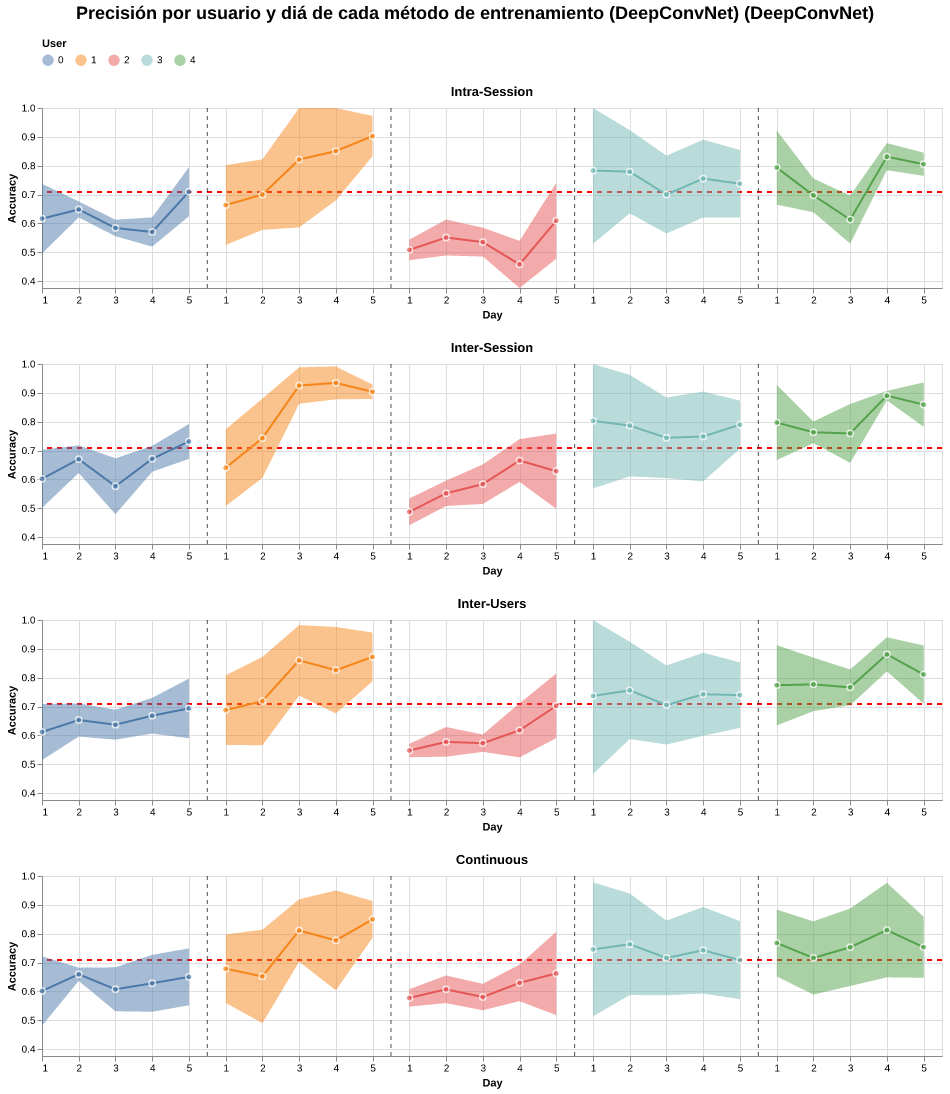
\includegraphics[width=1\textwidth]{img/resultados/Precision_por_usuario_y_dia_de_cada_metodo_de_entrenamiento_DeepConvNet_DeepConvNet.png}
  %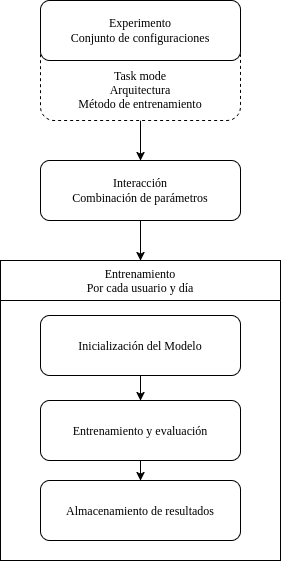
\includegraphics[height=\dimexpr\pagegoal-\pagetotal-\baselineskip\relax,width=\textwidth,keepaspectratio]{img/diagrama_pipeline.drawio.png}
  \caption{Variabilidad entre usuarios y día para cada método de entrenamiento para DeepConvNet.}
  \label{fig:user_day_variability_DeepConvNet}
\end{figure}

\begin{figure}[htbp]
  \centering
  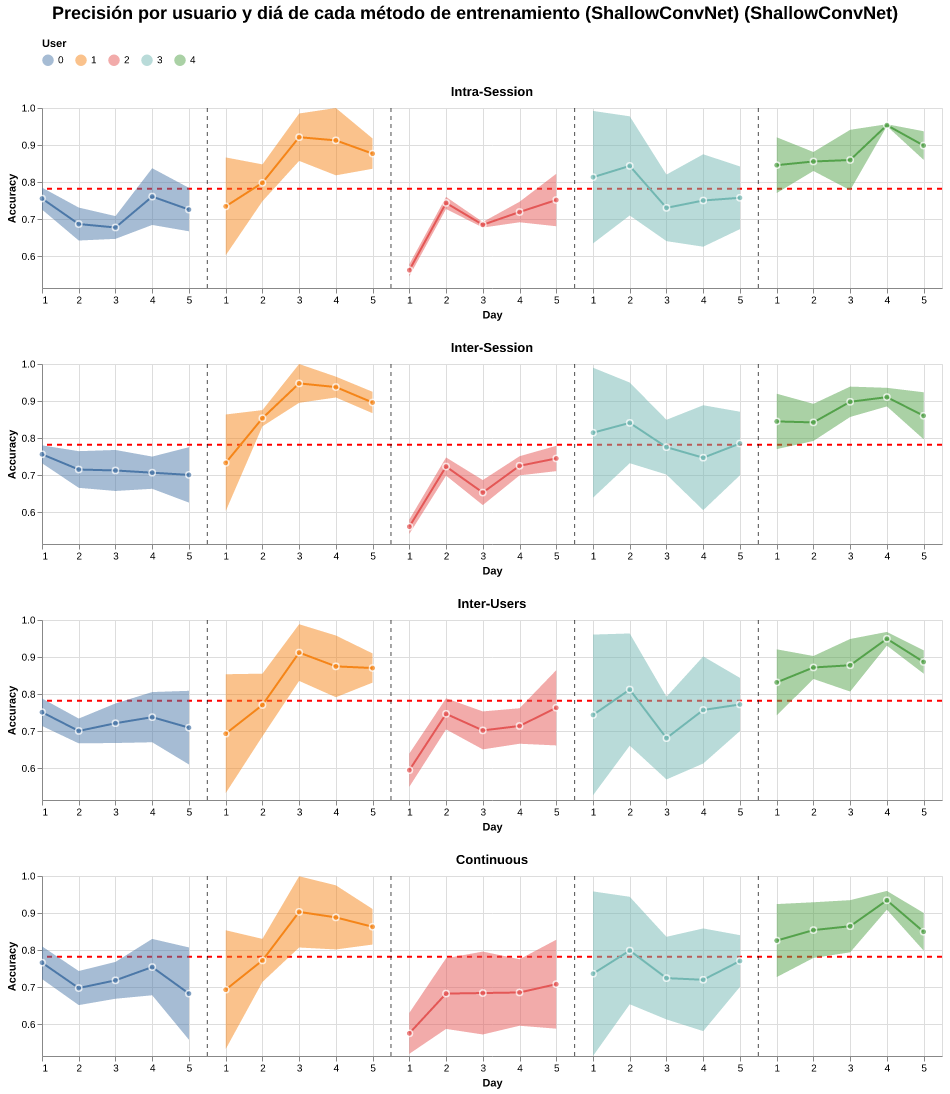
\includegraphics[width=1\textwidth]{img/resultados/Precision_por_usuario_y_dia_de_cada_metodo_de_entrenamiento_ShallowConvNet_ShallowConvNet.png}
  %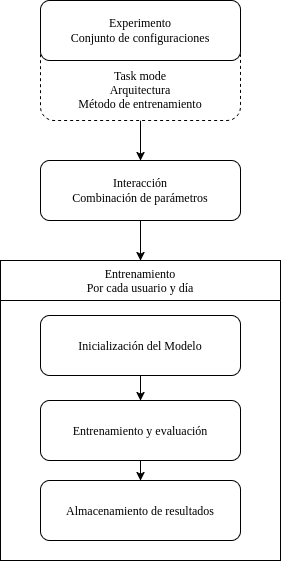
\includegraphics[height=\dimexpr\pagegoal-\pagetotal-\baselineskip\relax,width=\textwidth,keepaspectratio]{img/diagrama_pipeline.drawio.png}
  \caption{Variabilidad entre usuarios y día para cada método de entrenamiento para ShallowConvNet.}
  \label{fig:user_day_variability_ShallowConvNet}
\end{figure}

\begin{figure}[htbp]
  \centering
  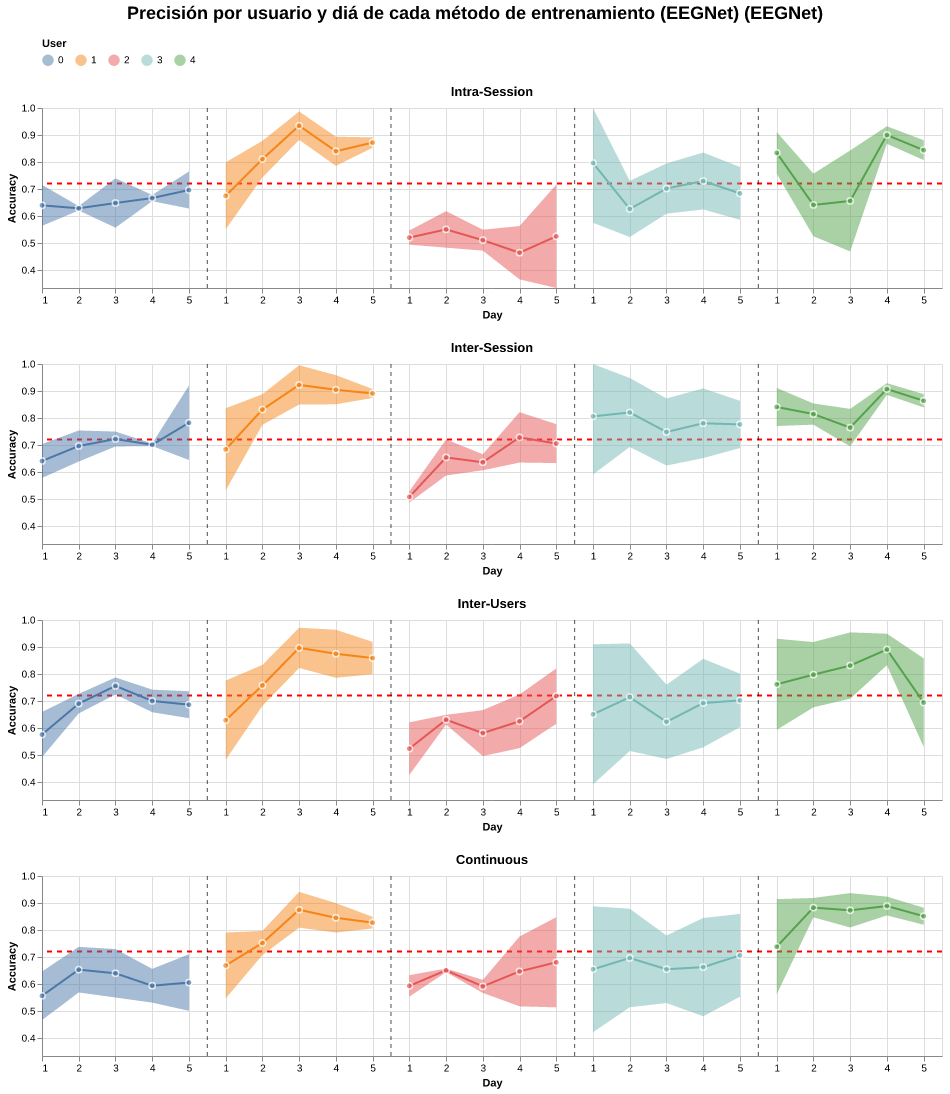
\includegraphics[width=1\textwidth]{img/resultados/Precision_por_usuario_y_dia_de_cada_metodo_de_entrenamiento_EEGNet_EEGNet.png}
  %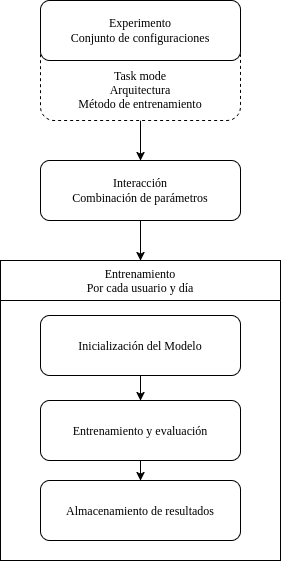
\includegraphics[height=\dimexpr\pagegoal-\pagetotal-\baselineskip\relax,width=\textwidth,keepaspectratio]{img/diagrama_pipeline.drawio.png}
  \caption{Variabilidad entre usuarios y día para cada método de entrenamiento para EEGNet.}
  \label{fig:user_day_variability_EEGNet}
\end{figure}


\newpage

\subsection{Queries complementarias}\label{sec:anexo_queries}

Con el objetivo de facilitar la reproducibilidad del análisis, el repositorio asociado al trabajo contiene las consultas SQL empleadas para obtener las tablas agregadas y generar las figuras presentadas en la memoria. En este anexo se incluyen las consultas principales, mientras que el conjunto completo puede consultarse en el directorio correspondiente del repositorio.

\subsubsection{Filtrado de Outliers}\label{sec:anexo_outliers}

Para realizar el filtrado de outliers utilizando el método Z-Score, se han definido nuevas vistas sobre cada una de las tablas \textbf{Runs\_t}, \textbf{Trials\_t} y \textbf{Classes\_t}. Manteniendo la estructura, pero eliminando valores atípicos. Además, se añaden los campos referentes a la configuración utilizada para el entrenamiento, de manera que se mantiene todo en la misma tabla.

Las queries utilizadas para la creación de las nuevas tablas ``limpias'' son las siguientes:

\begin{lstlisting}[
    style=sqlstyle,
    caption={Queries para la creación de las tablas ``limpias''.},
    label={cod:media_tarea}
]
CREATE
OR REPLACE VIEW runs_clean_z AS
WITH
    task_statistics AS (
        SELECT
            task_mode,
            AVG(acc1) AS mean_acc1,
            STDDEV_SAMP(acc1) AS std_acc1
        FROM
            runs_t
        WHERE
            acc1 IS NOT NULL
        GROUP BY
            task_mode
    )
SELECT
    t.*,
    p.*,
    (t.acc1 - s.mean_acc1) / NULLIF(s.std_acc1, 0) AS z_score
FROM
    runs_t AS t
    JOIN params_t AS p ON t.run_id = p.run_id
    JOIN task_statistics AS s ON t.task_mode = s.task_mode
WHERE
    t.acc1 IS NOT NULL
    AND t.acc1 <= 1
    AND ABS((t.acc1 - s.mean_acc1) / NULLIF(s.std_acc1, 0)) <= 3;

CREATE
OR REPLACE VIEW trials_clean_z AS
WITH
    task_statistics AS (
        SELECT
            task_mode,
            AVG(acc1) AS mean_acc1,
            STDDEV_SAMP(acc1) AS std_acc1
        FROM
            trials_t
        WHERE
            acc1 IS NOT NULL
        GROUP BY
            task_mode
    )
SELECT
    t.*,
    p.*,
    (t.acc1 - s.mean_acc1) / NULLIF(s.std_acc1, 0) AS z_score
FROM
    trials_t AS t
    JOIN params_t AS p ON t.run_id = p.run_id
    JOIN task_statistics AS s ON t.task_mode = s.task_mode
WHERE
    t.acc1 IS NOT NULL
    AND t.acc1 <= 1
    AND ABS((t.acc1 - s.mean_acc1) / NULLIF(s.std_acc1, 0)) <= 3;

CREATE
OR REPLACE VIEW classes_clean_z AS
WITH
    task_statistics AS (
        SELECT
            task_mode,
            AVG(precision) AS mean_acc1,
            STDDEV_SAMP(precision) AS std_acc1
        FROM
            classes_t
        WHERE
            precision IS NOT NULL
        GROUP BY
            task_mode
    )
SELECT
    t.*,
    p.*,
    (t.precision - s.mean_acc1) / NULLIF(s.std_acc1, 0) AS z_score
FROM
    classes_t AS t
    JOIN params_t AS p ON t.run_id = p.run_id
    JOIN task_statistics AS s ON t.task_mode = s.task_mode
WHERE
    t.precision IS NOT NULL
    AND t.precision <= 1
    AND ABS(
        (t.precision - s.mean_acc1) / NULLIF(s.std_acc1, 0)
    ) <= 3;
\end{lstlisting}




%%%%%%%%%%%%%%%%%%%%%%%%%%%%%%%%%%%%%%%%%%%%%%%%%%


%%%%%%%%%%%%%% - FIN DEL DOCUMENTO - %%%%%%%%%%%%%
\begin{sloppypar}
interwordspace: \the\fontdimen2\font \\

interwordstretch: \the\fontdimen3\font \\

emergencystretch: \the\emergencystretch\par

\end{sloppypar}
\end{document}

%%%%%%%%%%%%%%%%%%%%%%%%%%%%%%%%%%%%%%%%%%%%%%%%%%
